% Options for packages loaded elsewhere
\PassOptionsToPackage{unicode}{hyperref}
\PassOptionsToPackage{hyphens}{url}
%
\documentclass[
  man, donotrepeattitle,floatsintext]{apa7}
\usepackage{amsmath,amssymb}
\usepackage{iftex}
\ifPDFTeX
  \usepackage[T1]{fontenc}
  \usepackage[utf8]{inputenc}
  \usepackage{textcomp} % provide euro and other symbols
\else % if luatex or xetex
  \usepackage{unicode-math} % this also loads fontspec
  \defaultfontfeatures{Scale=MatchLowercase}
  \defaultfontfeatures[\rmfamily]{Ligatures=TeX,Scale=1}
\fi
\usepackage{lmodern}
\ifPDFTeX\else
  % xetex/luatex font selection
\fi
% Use upquote if available, for straight quotes in verbatim environments
\IfFileExists{upquote.sty}{\usepackage{upquote}}{}
\IfFileExists{microtype.sty}{% use microtype if available
  \usepackage[]{microtype}
  \UseMicrotypeSet[protrusion]{basicmath} % disable protrusion for tt fonts
}{}
\makeatletter
\@ifundefined{KOMAClassName}{% if non-KOMA class
  \IfFileExists{parskip.sty}{%
    \usepackage{parskip}
  }{% else
    \setlength{\parindent}{0pt}
    \setlength{\parskip}{6pt plus 2pt minus 1pt}}
}{% if KOMA class
  \KOMAoptions{parskip=half}}
\makeatother
\usepackage{xcolor}
\usepackage{graphicx}
\makeatletter
\def\maxwidth{\ifdim\Gin@nat@width>\linewidth\linewidth\else\Gin@nat@width\fi}
\def\maxheight{\ifdim\Gin@nat@height>\textheight\textheight\else\Gin@nat@height\fi}
\makeatother
% Scale images if necessary, so that they will not overflow the page
% margins by default, and it is still possible to overwrite the defaults
% using explicit options in \includegraphics[width, height, ...]{}
\setkeys{Gin}{width=\maxwidth,height=\maxheight,keepaspectratio}
% Set default figure placement to htbp
\makeatletter
\def\fps@figure{htbp}
\makeatother
\setlength{\emergencystretch}{3em} % prevent overfull lines
\providecommand{\tightlist}{%
  \setlength{\itemsep}{0pt}\setlength{\parskip}{0pt}}
\setcounter{secnumdepth}{-\maxdimen} % remove section numbering
% Make \paragraph and \subparagraph free-standing
\ifx\paragraph\undefined\else
  \let\oldparagraph\paragraph
  \renewcommand{\paragraph}[1]{\oldparagraph{#1}\mbox{}}
\fi
\ifx\subparagraph\undefined\else
  \let\oldsubparagraph\subparagraph
  \renewcommand{\subparagraph}[1]{\oldsubparagraph{#1}\mbox{}}
\fi
\newlength{\cslhangindent}
\setlength{\cslhangindent}{1.5em}
\newlength{\csllabelwidth}
\setlength{\csllabelwidth}{3em}
\newlength{\cslentryspacingunit} % times entry-spacing
\setlength{\cslentryspacingunit}{\parskip}
\newenvironment{CSLReferences}[2] % #1 hanging-ident, #2 entry spacing
 {% don't indent paragraphs
  \setlength{\parindent}{0pt}
  % turn on hanging indent if param 1 is 1
  \ifodd #1
  \let\oldpar\par
  \def\par{\hangindent=\cslhangindent\oldpar}
  \fi
  % set entry spacing
  \setlength{\parskip}{#2\cslentryspacingunit}
 }%
 {}
\usepackage{calc}
\newcommand{\CSLBlock}[1]{#1\hfill\break}
\newcommand{\CSLLeftMargin}[1]{\parbox[t]{\csllabelwidth}{#1}}
\newcommand{\CSLRightInline}[1]{\parbox[t]{\linewidth - \csllabelwidth}{#1}\break}
\newcommand{\CSLIndent}[1]{\hspace{\cslhangindent}#1}
\ifLuaTeX
\usepackage[bidi=basic]{babel}
\else
\usepackage[bidi=default]{babel}
\fi
\babelprovide[main,import]{english}
% get rid of language-specific shorthands (see #6817):
\let\LanguageShortHands\languageshorthands
\def\languageshorthands#1{}
% Manuscript styling
\usepackage{upgreek}
\captionsetup{font=singlespacing,justification=justified}

% Table formatting
\usepackage{longtable}
\usepackage{lscape}
% \usepackage[counterclockwise]{rotating}   % Landscape page setup for large tables
\usepackage{multirow}		% Table styling
\usepackage{tabularx}		% Control Column width
\usepackage[flushleft]{threeparttable}	% Allows for three part tables with a specified notes section
\usepackage{threeparttablex}            % Lets threeparttable work with longtable

% Create new environments so endfloat can handle them
% \newenvironment{ltable}
%   {\begin{landscape}\centering\begin{threeparttable}}
%   {\end{threeparttable}\end{landscape}}
\newenvironment{lltable}{\begin{landscape}\centering\begin{ThreePartTable}}{\end{ThreePartTable}\end{landscape}}

% Enables adjusting longtable caption width to table width
% Solution found at http://golatex.de/longtable-mit-caption-so-breit-wie-die-tabelle-t15767.html
\makeatletter
\newcommand\LastLTentrywidth{1em}
\newlength\longtablewidth
\setlength{\longtablewidth}{1in}
\newcommand{\getlongtablewidth}{\begingroup \ifcsname LT@\roman{LT@tables}\endcsname \global\longtablewidth=0pt \renewcommand{\LT@entry}[2]{\global\advance\longtablewidth by ##2\relax\gdef\LastLTentrywidth{##2}}\@nameuse{LT@\roman{LT@tables}} \fi \endgroup}

% \setlength{\parindent}{0.5in}
% \setlength{\parskip}{0pt plus 0pt minus 0pt}

% Overwrite redefinition of paragraph and subparagraph by the default LaTeX template
% See https://github.com/crsh/papaja/issues/292
\makeatletter
\renewcommand{\paragraph}{\@startsection{paragraph}{4}{\parindent}%
  {0\baselineskip \@plus 0.2ex \@minus 0.2ex}%
  {-1em}%
  {\normalfont\normalsize\bfseries\itshape\typesectitle}}

\renewcommand{\subparagraph}[1]{\@startsection{subparagraph}{5}{1em}%
  {0\baselineskip \@plus 0.2ex \@minus 0.2ex}%
  {-\z@\relax}%
  {\normalfont\normalsize\itshape\hspace{\parindent}{#1}\textit{\addperi}}{\relax}}
\makeatother

% \usepackage{etoolbox}
\makeatletter
\patchcmd{\HyOrg@maketitle}
  {\section{\normalfont\normalsize\abstractname}}
  {\section*{\normalfont\normalsize\abstractname}}
  {}{\typeout{Failed to patch abstract.}}
\patchcmd{\HyOrg@maketitle}
  {\section{\protect\normalfont{\@title}}}
  {\section*{\protect\normalfont{\@title}}}
  {}{\typeout{Failed to patch title.}}
\makeatother

\usepackage{xpatch}
\makeatletter
\xapptocmd\appendix
  {\xapptocmd\section
    {\addcontentsline{toc}{section}{\appendixname\ifoneappendix\else~\theappendix\fi\\: #1}}
    {}{\InnerPatchFailed}%
  }
{}{\PatchFailed}
\keywords{Skill acquisition, OPTIMAL theory, Metascience, Heterogeneity, Sport Science
}
\usepackage{lineno}

\linenumbers
\usepackage{csquotes}
\raggedbottom
\usepackage{sectsty}
\sectionfont{\centering\normalfont\normalsize\bfseries}
\subsectionfont{\normalfont\normalsize\bfseries\itshape}
\subsubsectionfont{\normalfont\normalsize\itshape}
\usepackage{censor}
\usepackage{graphicx}
\ifLuaTeX
  \usepackage{selnolig}  % disable illegal ligatures
\fi
\IfFileExists{bookmark.sty}{\usepackage{bookmark}}{\usepackage{hyperref}}
\IfFileExists{xurl.sty}{\usepackage{xurl}}{} % add URL line breaks if available
\urlstyle{same}
\hypersetup{
  pdftitle={Reporting bias, not external focus: A robust Bayesian meta-analysis of the attentional focus literature},
  pdflang={en-EN},
  pdfkeywords={Skill acquisition, OPTIMAL theory, Metascience, Heterogeneity, Sport Science},
  hidelinks,
  pdfcreator={LaTeX via pandoc}}

\title{Reporting bias, not external focus: A robust Bayesian meta-analysis of the attentional focus literature}
\author{\textsuperscript{}}
\date{}


\shorttitle{Reporting bias, not external focus}

\authornote{

\vspace{-0.5cm}

\noindent Data and code: \url{https://osf.io/vfmx2/?view_only=002325d59dd64562a20301167240f0f9}

}

\affiliation{\phantom{0}}

\abstract{%
Evidence has ostensibly been accumulating over the past two decades suggesting that an external focus of attention is superior to an internal focus for the performance and learning of motor skills. Seven previous meta-studies have all reported evidence of external focus superiority---the most comprehensive of which concluded the benefits apply to motor skill (a) retention, (b) transfer, and (c) performance; results in (d) reduced electromyographic activity during performance, and that (e) more distal external foci are superior to proximal external foci for performance. Here, we re-analyzed these data using robust Bayesian meta-analysis methods that included several plausible models of publication bias. We found moderate to strong evidence of publication bias for all five analyses. After correcting for publication bias, estimated mean effects were negligible: \emph{g} = .01 (performance), \emph{g} = .15 (retention), \emph{g} = .09 (transfer), \emph{g} = .06 (electromyography), and \emph{g} = -.01 (distance effect). Bayes factors indicated data favored the null for each analysis, ranging from BF\textsubscript{01} = 1.3 (retention) to 5.75 (performance). Further, we found clear evidence of heterogeneity in each analysis, suggesting the impact of attentional focus depends on yet unknown contextual factors. Our results contradict the existing consensus that an external focus is always more effective than an internal focus. Instead, focus of attention appears to have a variety of effects that we cannot account for, and on average those effects are small to nil. These results parallel previous metascience suggesting publication bias has obfuscated the motor learning literature.
}



\begin{document}
\maketitle

\noindent \textbf{\emph{Public Significance Statement}}\\
\noindent A robust Bayesian meta-analysis showed that directing learners to focus their attention on their intended movement effects---often called an external focus---may have little-to-no effect on motor performance and learning on average. While the consensus among researchers and practitioners has been that an external focus is superior to focusing on one's own body during practice, the present results suggest this may depend on unknown factors and our current understanding has been distorted by publication bias.

\newpage

Where should you focus when performing and/or learning a motor skill? The most basic of questions for a novice learner and an experienced performer alike. Is it better to focus on what you are doing: where your body is in space and how it is behaving? Or is it better to focus on what you intend to do: the end effect you are trying to achieve independent of how your body achieves it? This question has been the topic of decades of research comparing an internal focus of attention (i.e., focusing on your own body) to an external focus of attention (i.e., focusing on the intended effect of the action). Gabriele Wulf pioneered this area of inquiry in 1998, publishing a two-experiment paper illustrating the benefits of adopting an external focus (Wulf, Höß, \& Prinz, 1998). In the experiments, instructing learners to focus on the wheels of a ski simulator (Experiment 1) or the markers on a balance platform (Experiment 2) led to improved motor learning compared to focusing on one's feet. Dozens of studies have since replicated these initial findings (see Wulf, 2007; Wulf, 2013 for reviews).

Previous reviews have argued that research shows benefits of an external focus in four main areas: (a) effectiveness at accuracy and balance tasks, (b) efficiency in electromyographic activity, force production, speed, and endurance tasks, (c) promoting automaticity, and (d) enhancing movement form (Chua, Jimenez-Diaz, Lewthwaite, Kim, \& Wulf, 2021; Wulf, 2007, 2013; Wulf \& Lewthwaite, 2016). A leading explanation for the mechanism causing these benefits is goal-action coupling: a process proposed in Wulf and Lewthwaite's (2016) OPTIMAL theory involving a shift at the neural level that simultaneously directs action toward success and stifles deleterious self-focused cognition. While focus of attention is fundamental to the OPTIMAL theory, various perspectives in motor behavior have offered complementary accounts for external focus benefits. For example, it has been argued from the constraints-based approach that an external focus promotes the search of the task during practice and provides a constraint on emerging actions (Davids, Araújo, Shuttleworth, \& Button, 2003). It has also been argued that actions and perceptions share a common (cognitive) code; therefore, focusing on the intended (perceptual) effect of an action is consistent with its underlying neural coding (Hommel, Müsseler, Aschersleben, \& Prinz, 2001; Prinz, 1990; Wulf \& Prinz, 2001). While research continues to explore the putative mechanisms, there is consensus in the motor learning community that adopting an external focus of attention can improve motor performance, retention, transfer, and movement efficiency---at least most of the time (Chua et al., 2021; Grgic, Mikulic, \& Mikulic, 2021; Grgic \& Mikulic, 2022; T. Kim, Jimenez-Diaz, \& Chen, 2017; Lee \& Carnahan, 2021; Li, Zhang, Yue, Memmert, \& Zhang, 2022; Hubert Makaruk, Starzak, \& Porter, 2020; Nicklas, Rein, Noël, \& Klatt, 2022).\footnote{While we acknowledge this as the general consensus in the field, it is important to note that there are mixed findings and alternative discussions in this area of research (e.g., Bernier, Trottier, Thienot, \& Fournier, 2016; Brick, MacIntyre, \& Campbell, 2014; Canning, 2005; Collins, Carson, \& Toner, 2016; Emanuel, Jarus, \& Bart, 2008; Lawrence, Gottwald, Hardy, \& Khan, 2011; Maurer \& Munzert, 2013; Peh, Chow, \& Davids, 2011; Perkins-Ceccato, Passmore, \& Lee, 2003; Schorer, Jaitner, Wollny, Fath, \& Baker, 2012; Zentgraf \& Munzert, 2009).}

Buttressed by the largely positive results in the research literature, external focus of attention is now widely recommended outside of academia, including by sport coaches (skating: Smale, 2021; golf: T. Neumann, 2017; tennis: Kuzdub, 2022; baseball: Peterson, 2019), fitness coaches (Kompf, 2015; N. Winkelman, 2015), and therapists (Lo, 2019; Magne \& Edge, 2017). Researchers continue to study the use of externally focused instructions and feedback in clinical settings (Johnson et al., 2023) and are currently developing strategies for increasing awareness of the research among rehabilitation professionals (Hussien, Gignac, Shearer, \& Ste-Marie, 2023a, 2023b; Hussien \& Ste-Marie, 2023). As external focus becomes evermore mainstream, recent concerns that much of the motor learning literature may be exaggerated by reporting bias (e.g., K. Lohse, Buchanan, \& Miller, 2016; McKay, Hussien, et al., 2022; McKay, Yantha, Hussien, Carter, \& Ste-Marie, 2022; Mesquida, Murphy, Lakens, \& Warne, 2022; Twomey et al., 2021) underlines the need for careful assessment of the evidence. The external focus literature may be especially at risk because substantial reporting bias has been found in the motor learning literature investigating the other factors within OPTIMAL theory (Bacelar, Parma, Murrah, \& Miller, 2022; McKay, Bacelar, Parma, Miller, \& Carter, 2023; McKay, Yantha, et al., 2022). Note that reporting bias encompasses various forms of selection bias that limit the availability of data. Potential reporting bias mechanisms can be modeled, though models cannot determine the specific reason for censorship within a literature.

\hypertarget{previous-meta-analyses}{%
\subsection{Previous meta-analyses}\label{previous-meta-analyses}}

There have been seven meta-analyses comparing the effects of internal and external focus instructions on motor outcomes. Five have focused on specific task-types: balance (T. Kim et al., 2017), jumping (Hubert Makaruk et al., 2020), sprinting (Li et al., 2022), strength (Grgic et al., 2021), and endurance (Grgic \& Mikulic, 2022). A sixth included all motor tasks and focused specifically on the immediate effect on performance (Nicklas et al., 2022). Chua and colleagues (2021) conducted the most comprehensive meta-analysis of the seven, including all task-types and estimating effects on performance, retention, transfer, electromyography activity, and the distance effect. All seven studies reported the results of random effects meta-analyses as the primary estimates for the effect of focus of attention. Although there was some variance in point estimates and confidence intervals, each of the studies reported evidence that an external focus is superior to an internal focus.

Importantly, a random effects model assumes no reporting bias and has been shown to be quite biased in the presence of selective reporting for statistical significance (Bartoš, Maier, Shanks, et al., 2023; Bom \& Rachinger, 2019; Carter, Kofler, Forster, \& McCullough, 2015; Carter, Schönbrodt, Gervais, \& Hilgard, 2019; Kvarven, Strømland, \& Johannesson, 2020; Stanley, Doucouliagos, \& Ioannidis, 2017, 2022). Two of the seven previous studies (Chua et al., 2021; T. Kim et al., 2017) reported evidence of funnel plot asymmetry, which is consistent with selective reporting of significant results. Two studies did not find evidence of funnel plot asymmetry (Li et al., 2022; Nicklas et al., 2022), and the other three did not investigate reporting bias at all (Grgic et al., 2021; Grgic \& Mikulic, 2022; Hubert Makaruk et al., 2020). Both studies that observed evidence of reporting bias conducted a fail-safe-style sensitivity analysis, but did not correct the primary estimates for the presence of bias. The meta-analysis by Chua et al. (2021) did calculate worst-case-scenario estimates based on a random effects meta-analysis of the non-significant results. Thus, although reporting bias may be prevalent in the field of motor learning (K. Lohse et al., 2016), and two previous meta-analyses have found evidence of reporting bias in the attentional focus literature (Chua et al., 2021; T. Kim et al., 2017), the primary estimates from all previous meta-analyses assume bias is absent.

Consistent with the other studies, Chua et al. (2021) reported moderate benefits of an external focus for learning measures (\emph{g} = .58) and small benefits for performance measures (\emph{g} = .26) and the distance effect (\emph{g} = .22). Chua and colleagues also reported a large effect on electromyography activity (\emph{g} = .83). In lieu of bias-corrected estimates, worst-case scenario estimates were calculated to evaluate how sensitive the primary estimates were to an assumed model of reporting bias. Under the assumed model, significant results in the predicted direction are published without censorship, while all non-significant results and significant results in the opposite direction are censored at the same rate. The worst-case scenario is simply the random effects estimate of all the non-preferred outcomes, since a preference for significant results in the predicted direction cannot upwardly bias an estimate if significant results are removed. If the worst-case scenario is positive, then one can conclude that no amount of reporting bias could attenuate the point estimate to the null value. However, this conclusion is only merited if censorship is entirely captured by the assumed model. If other plausible mechanisms of censorship are present, then the assumed model does not hold, and the worst-case scenario estimates can no longer be considered as such.

Although Chua et al. (2021) concluded that no amount of reporting bias could attenuate the effect to the null value for any measure (performance, retention, transfer, electromyography, and the distance effect), there are several plausible censorship mechanisms that were unexplored. For example, it is plausible that nearly significant results, often called non-significant trends (Otte, Vinkers, Habets, IJzendoorn, \& Tijdink, 2022), were censored less than other non-significant trends. It is also possible that point estimates favoring an internal focus were the least preferred result. If these plausible alternative censorship mechanisms were active in the attentional focus literature, then the random effects estimate of ``all non-significant in the predicted direction'' results would be positively biased. While Chua et al. (2021) concluded that external focus superiority is not sensitive to reporting bias, it remains unknown if that conclusion is sensitive to the form of reporting bias that was assumed.

\hypertarget{present-study}{%
\subsection{Present study}\label{present-study}}

Seven previous meta-analyses provide primary estimates of the potential benefit of an external focus of attention while assuming reporting bias is absent. Given the evidence of reporting bias reported in two of those studies (Chua et al., 2021; T. Kim et al., 2017), along with evidence of extensive bias in related literatures (e.g., K. Lohse et al., 2016; McKay et al., 2023), bias-corrected estimates are needed. There are several plausible mechanisms of reporting bias, and the true model is unknowable. Therefore, using a robust Bayesian approach to meta-analysis (Bartoš, Maier, Wagenmakers, Doucouliagos, \& Stanley, 2023), we leveraged Bayesian model-averaging to fit several plausible models of reporting bias to the attentional focus literature examined by Chua et al. (2021). Greater weight was given to the models that best accounted for the results and less weight was given to poorly performing models. This approach allowed us to calculate reporting-bias-adjusted estimates for the effect of attentional focus on motor learning, performance, electromyography activity, and for the distance effect. Our approach naturally allowed us to evaluate Chua and colleagues' (2021) claims that no amount of reporting bias could attenuate the effect to the null value.

In addition to censorship mechanisms, we also explored the role of \emph{post hoc} outcome selection leading to potentially exaggerated estimates. The previous seven meta-analyses either did not specify exactly how outcomes were selected for analysis (Grgic et al., 2021; Grgic \& Mikulic, 2022; T. Kim et al., 2017; Li et al., 2022; Hubert Makaruk et al., 2020), excluded studies that had more than one performance measurement unless the measures could be ranked and a primary measure could be selected (Nicklas et al., 2022), or selected the outcome positioned as primary in the original research article (Chua et al., 2021). The external focus literature has not made use of preregistration or Registered Reports, so it is possible that the most impressive results have sometimes been positioned as primary because they were the most impressive. If this sort of \emph{post hoc} selection is present, then selecting outcomes based on their status in the original article may lead to biased estimates. To evaluate the possibility of \emph{post hoc} selection bias, we extracted effect size estimates for the retention test outcomes that were not selected by Chua et al. (2021), but could have been, and compared them to the selected ``primary'' outcomes.

In the present study, we addressed the following questions: (a) What is the reporting-bias-adjusted estimate for the effect of attentional focus on learning, performance, electromyography activity, and the distance effect? (b) How sensitive are random effects estimates to the assumption that reporting bias is absent? (c) How sensitive are Chua and colleagues' (2021) conclusions that no amount of reporting bias could attenuate the effect to the null value to the specific model of censorship that was evaluated? and (d) How influential was \emph{post hoc} selection bias on the estimated benefits of an external focus of attention on retention performance?

\hypertarget{methods}{%
\section{Methods}\label{methods}}

\hypertarget{transparency-and-openness}{%
\subsection{Transparency and openness}\label{transparency-and-openness}}

We adhered to the MARS guidelines for meta-analytic reporting (Appelbaum et al., 2018). The data, code, and preregistration for this study can be found here: \url{https://osf.io/vfmx2/?view_only=002325d59dd64562a20301167240f0f9}. The data for each primary outcome measure were collected and reported by Chua et al. (2021). Our re-analysis of those data was not preregistered as we were already aware of Chua and colleagues' (2021) primary conclusions and had seen the data visualizations in their study. Data for up to three additional outcomes from each experiment that examined retention test performance were collected and analyzed according to our preregistered protocol.

Statistical analyses were conducted using R (Version 4.3.2; R Core Team, 2023) and the R-packages \emph{compute.es} (Version 0.2.5; Re, 2013), \emph{daff} (Version 0.3.5; Fitzpatrick, de Jonge, \& Warnes, 2019), \emph{extrafont} (Version 0.19; Chang, 2023), \emph{faux} (Version 1.2.1; DeBruine, 2023), \emph{ggdist} (Version 3.2.1; Kay, 2023), \emph{ggplot2} (Version 3.4.1; Wickham, 2016), \emph{gt} (Version 0.9.0; Iannone et al., 2023), \emph{kableExtra} (Version 1.3.4; Zhu, 2021), \emph{magick} (Version 2.7.4; Ooms, 2023), \emph{metafor} (Version 4.0.0; Viechtbauer, 2010), \emph{papaja} (Version 0.1.1.9001; Aust \& Barth, 2020), \emph{patchwork} (Version 1.1.2; Pedersen, 2022), \emph{plotly} (Version 4.10.2; Sievert, 2020), \emph{PublicationBias} (Version 2.3.0; Braginsky, Mathur, \& VanderWeele, 2023), \emph{renv} (Version 0.17.2; Ushey, 2023), \emph{RoBMA} (Version 2.3.2; Bartoš \& Maier, 2020), \emph{stringi} (Version 1.7.12; Gagolewski, 2022), \emph{tidyverse} (Version 2.0.0; Wickham et al., 2019), and \emph{tinylabels} (Version 0.2.3; Barth, 2022) were used in this project.

\hypertarget{eligibility}{%
\subsection{Eligibility}\label{eligibility}}

Our analysis was restricted to the studies included in the study by Chua et al. (2021), meaning our study inherits the inclusion criteria imposed in their study: (a) published in English between February 1998 and April 2019, (b) in a peer-reviewed journal, (c) compared internal and external foci of attention, or at least two types of external focus, (d) measured motor learning or performance, (e) used a within-participant design to measure performance and a between participants design to measure learning, (f) included sufficient data to calculate effect sizes, and (g) were experiments.

\hypertarget{data-collection-process}{%
\subsection{Data collection process}\label{data-collection-process}}

The data reported by Chua et al. (2021) were extracted directly from the published article. Additionally, up to three outcomes were extracted from each experiment included in the meta-analysis of retention test performance.\footnote{We chose to focus on retention effects because the performance estimates were already small. The retention estimates were substantial, and retention tests are often the focal learning measure in an experiment. Almost all transfer tests were from studies that also included a retention test, so focusing on retention outcomes was the simplest way to test our research question.} Data were extracted in duplicate by a team of six researchers working independently (AC, JS, CDF, HH, KA, FA). The lead author evaluated each pair of extractions using the \texttt{R} package \texttt{daff} (Fitzpatrick et al., 2019) for consensus and resolved all conflicts.

Outcome measures were selected for extraction based on our preregistered priority list (see Table \ref{tab:table1}). A priority list achieved two goals. First, it prevented selection bias when several outcomes were reported in a study by establishing which outcomes to select \emph{a priori}. Second, the list prioritized outcomes most connected to the goal of the task over outcomes only correlated with success. This ensured the dependent variables most indicative of goal-action coupling were selected from each study.

\begin{table}

\caption{\label{tab:table1}Priority list for extracting outcome measures.}
\fontsize{10}{12}\selectfont
\begin{tabular}[t]{clcl}
\toprule
Priority & Measure & Priority & Measure\\
\midrule
1 & Absolute error & 6 & Relative timing error\\
2 & Root mean squared error / Total error & 7 & Absolute constant error\\
3 & Accuracy points & 8 & Movement time\\
4 & Variable error & 9 & Movement form (Expert raters)\\
5 & Absolute timing error & 10 & Other\\
\bottomrule
\end{tabular}
\end{table}

The sample sizes, direction of effect, means, and standard deviations were extracted for each measure when available. If standard deviations were not reported, data were extracted in the following order of priority: means and standard errors, \emph{F}-values, then \emph{t}-values. If the required data were not reported in the text of the article, but were presented in figures with error bars, then the mean and standard deviation were extracted by digitizing the plots (Rohatgi, 2022). Data from six studies were digitized. If data could not be extracted with plot digitization, then the authors were emailed, and the data were requested. If the authors did not respond, a follow up email was sent. Emails were sent to authors requesting data for five effects, and one author responded with the requested data. Hedges' \emph{g} for the newly extracted outcomes was calculated using the \texttt{R} package \texttt{compute.es} (Re, 2013). Risk of bias from methodological weaknesses was well probed by Chua et al. (2021) and was not revisited in this study.

\hypertarget{synthesis-methods}{%
\subsection{Synthesis methods}\label{synthesis-methods}}

\hypertarget{influential-cases}{%
\subsubsection{Influential cases}\label{influential-cases}}

We screened the data for influential cases using the \texttt{R} package \texttt{metafor} (Viechtbauer, 2010). After fitting univariate random effects models for each meta-analysis, externally standardized residuals and Cook's distances were calculated. Studies identified as extreme by both measures were considered influential and a sensitivity analysis was conducted with the studies removed.\footnote{Our approach to influential case screening differed from the approach employed by Chua et al. (2021) and we therefore arrived at a different number of outliers for each analysis (see Supplementary A for more details).}

\hypertarget{reporting-bias}{%
\subsubsection{Reporting bias}\label{reporting-bias}}

We implemented a robust Bayesian approach (Bartoš, Maier, Wagenmakers, et al., 2023) to reanalyze the five meta-analyses reported by Chua et al. (2021). We used neutral default priors for the presence of an effect (Normal(M = 0, SD = 1), \emph{p} = .5), the presence of heterogeneity (InvGamma(1, 0.15), \emph{p} = .5), and the presence of reporting bias (\emph{p} = .5). Reporting bias was probed using selection models and funnel plot regression models. In the selection model class, six different weight-function models were fit to model censorship based on specific \emph{p}-value thresholds. For example, one selection model captures the possibility that significant results in the predicted direction are more likely to survive to be published than both null results and significant results in the unpredicted direction. Another selection model captures the possibility that results in the unpredicted direction are the least likely to survive censorship, while non-significant trends are more likely than other null results, but not as likely as significant results to survive.

A total of six selection models capturing different plausible censorship scenarios are assigned half of the prior probability that reporting bias exists. The other half of the prior probability is allocated to funnel plot regression models. The precision-effect test (PET) and precision-effect estimate with standard errors (PEESE) respectively model a linear and quadratic relationship between standard error and effect size. If the data were censored such that lower \emph{p}-values had a higher probability of surviving, a correlation would emerge between two otherwise independent causes of \emph{p}-values: effect sizes and standard errors. The PET method fits a linear relationship between effect size and standard error, modeling a consistent level of censorship across studies. The PEESE method fits a quadratic relationship, reflecting the possibility that studies with small standard errors, and thus large samples, are likely to be reported regardless of the results, while small studies with large standard errors require increasingly impressive results to garner publication.\footnote{Priors for the six selection models were: \(\omega\){[}two-sided: .05{]} \(\sim\) CumDirichlet(1, 1), \(\omega\){[}two-sided: .1, .05{]} \(\sim\) CumDirichlet(1, 1, 1), \(\omega\){[}one-sided: .05{]} \(\sim\) CumDirichlet(1, 1), \(\omega\){[}one-sided: .05, .025{]} \(\sim\) CumDirichlet(1, 1, 1), \(\omega\){[}one-sided: .5, .05{]} \(\sim\) CumDirichlet(1, 1, 1), \(\omega\){[}one-sided: .5, .05, .025{]} \(\sim\) CumDirichlet(1, 1, 1, 1). Priors for the two regression models were: PET \(\sim\) Cauchy(0, 1){[}0, Inf{]}, PEESE \(\sim\) Cauchy(0, 5){[}0, Inf{]}.}

A total of 36 models were fit to the data with every combination of the eight reporting bias models, models assuming an effect, no effect, heterogeneity, no heterogeneity, and no reporting bias (see Supplementary B for more details). The estimates of each model were combined using Bayesian model-averaging, where model estimates are weighted based on how well the model fit the data. A single posterior distribution was generated for the average effect of an external focus and the average value of \emph{tau}---the estimated heterogeneity. Further, Bayes Factors were calculated measuring the evidence in favor of an effect, the presence of heterogeneity, and reporting bias.

\hypertarget{post-hoc-selection-bias}{%
\subsubsection{Post-hoc selection bias}\label{post-hoc-selection-bias}}

A multi-level mixed effects model with outcomes nested in study, and with cluster-robust standard errors compared the outcomes selected by Chua et al. (2021) to the additional outcomes that might have been selected instead. Profile analysis was conducted to ensure the model converged on unique solutions for estimates of \emph{Mu} (the mean effect of external focus in the population) and \emph{tau}.

\hypertarget{results}{%
\section{Results}\label{results}}

Model-averaged posterior distributions for each analysis with and without outliers are presented in Figure \ref{fig:fig1}.\footnote{Model convergence diagnostics were conducted for all RoBMA analyses. In each case, Rhat convergence values were less than 1.05 and effect sampling sizes were a few hundred or more.}

\hypertarget{performance}{%
\subsection{Performance}\label{performance}}

Influence analyses revealed four studies (Marchant, Greig, et al., 2009; Nadzalan et al., 2015; Porter, Nolan, et al., 2010; Sherwood et al., 2014; Exp 1 and 2) could be considered outliers in the performance meta-analysis. We report the results with all studies included first, then with outliers removed. The mean of the model-averaged posterior distribution for the difference between external and internal foci of attention on motor skill performance was \emph{g} = 0.01, 95\% credible interval: 0, 0.17. The data were over 5 times more compatible with the null hypothesis than the alternative, BF\textsubscript{10} = 0.17. There was clear evidence of heterogeneity, \(\tau\) = 0.40, BF\textsubscript{rf} = Infinite. There was also clear evidence of publication bias, BF\textsubscript{pb}=162,651.73. Removing influential cases did not substantively change the conclusions: \emph{g} = 0.02, 95\% credible interval: 0, 0.16, BF\textsubscript{10} =0.26; \(\tau\) =0.25, BF\textsubscript{rf} = 602774614; BF\textsubscript{pb} = 97,268.05.

\clearpage

\begin{figure}

{\centering 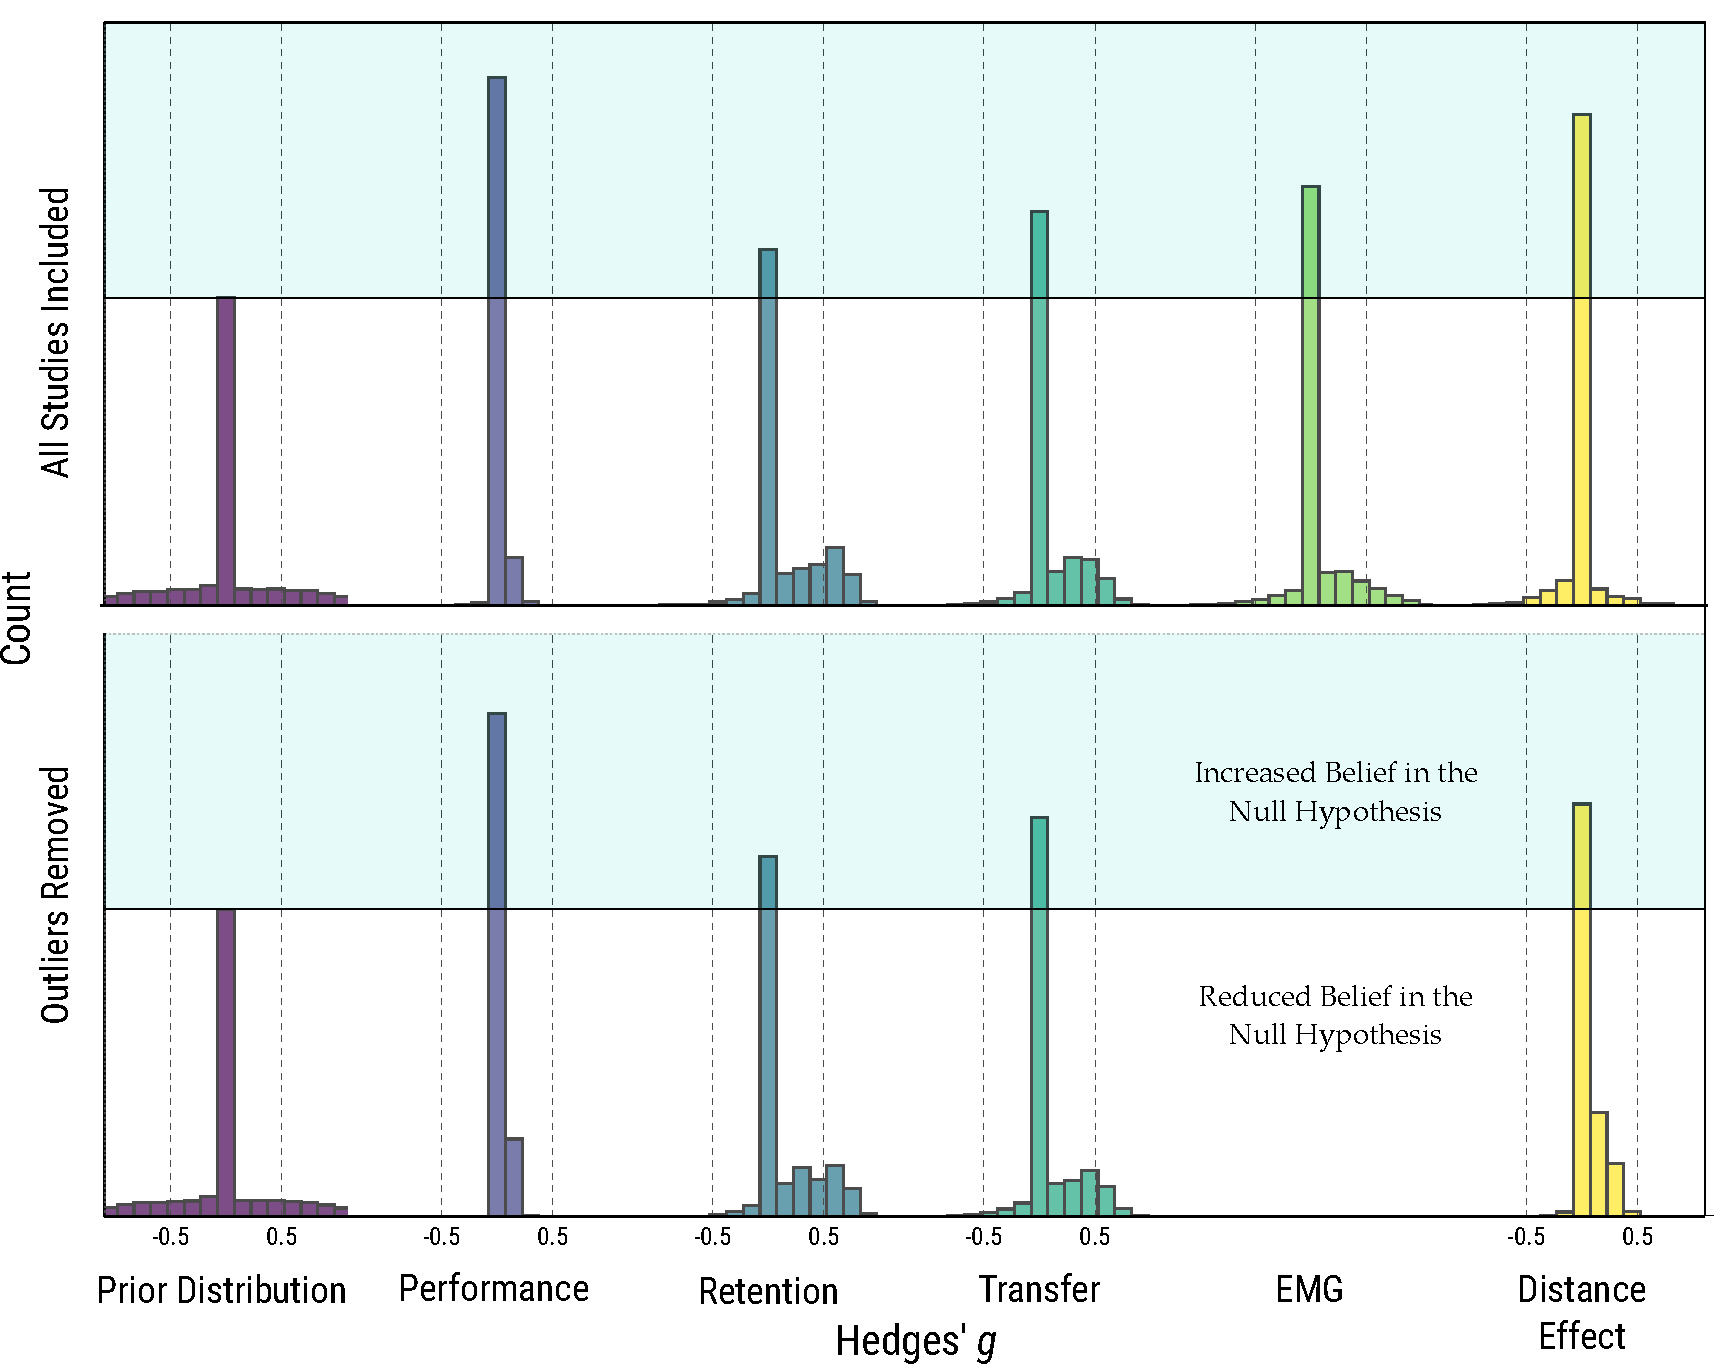
\includegraphics{../../figs/fig1} 

}

\caption{\linespread{1.15}\selectfont \small \normalfont \textbf{Posterior plots of the standardized mean difference with and without outliers.} The effect size estimates (\emph{g}) of each meta-analysis with all studies included (top row) and with outliers removed (bottom row). The histograms in the first column reflect the prior distribution, with 50\% of the probability density concentrated on zero effect (the null hypothesis) and 50\% of the density normally distributed (\emph{M} = 0, \emph{SD} = 1). The model-averaged posterior distributions for performance, retention, transfer, electromyography, and the distance effect are presented in the second through sixth columns, respectively. Increased belief in the null hypothesis is visible for each analysis, illustrated by the increased height of the spike at \emph{g} = 0 in all posteriors relative to the prior distribution.}\label{fig:fig1}
\end{figure}



\clearpage

\hypertarget{retention}{%
\subsection{Retention}\label{retention}}

Two studies (Ahmad et al.~2013; Tse, 2017) were identified as possible outliers in the retention test meta-analysis. Again, the results with all studies included are reported first, then with outliers removed. The mean of the model-averaged posterior distribution for the effect of focus of attention on retention was \emph{g} = 0.15, 95\% credible interval: -0.17, 0.74. The data were somewhat more consistent with the null hypothesis than the alternative, BF\textsubscript{10} = 0.75. There was clear evidence of heterogeneity, \(\tau\) = 0.65, BF\textsubscript{rf} = Infinite. The data were 5.9 times more compatible with models assuming publication bias than without, BF\textsubscript{pb} = 5.92. Removing two influential cases did not substantively change the conclusions: \emph{g} = 0.14, 95\% credible interval: -0.18, 0.73, BF\textsubscript{10}=0.73; \(\tau\) =0.50, BF\textsubscript{rf} = 1,688,117,430.52; BF\textsubscript{pb} = 7.62.

\hypertarget{transfer}{%
\subsection{Transfer}\label{transfer}}

One possible outlier (Tse, 2017) was identified in the transfer test meta-analysis. The mean of the model-averaged posterior distribution of all transfer outcomes was \emph{g} = 0.09, 95\% credible interval: -0.21, 0.62. The results were somewhat more likely under the null hypothesis than the alternative, BF\textsubscript{10} = 0.57. There was clear evidence of heterogeneity, \(\tau\) = 0.56, BF\textsubscript{rf} = Infinite. The data were more than 6.4 times more likely under models assuming publication bias, BF\textsubscript{pb} = 6.45. Removing one influential case did not substantively change the conclusions: \emph{g} = 0.09, 95\% credible interval: -0.23, 0.63, BF\textsubscript{10} = 0.55; \(\tau\) = 0.45, BF\textsubscript{rf} = 101,220.12; BF\textsubscript{pb} = 9.06.

\hypertarget{electromyography}{%
\subsection{Electromyography}\label{electromyography}}

There were no outliers identified in the electromyography meta-analysis. The mean of the model-averaged posterior distribution for the effect of attentional focus on electromyography activity was \emph{g} = 0.06, 95\% credible interval: -0.35, 0.69. The data were twice as likely under the null hypothesis as the alternative, BF\textsubscript{10} = 0.47. There was clear evidence of heterogeneity, \(\tau\) = 0.49, BF\textsubscript{rf} = Infinite. There was very strong evidence of publication bias, BF\textsubscript{pb} = 26.40.

\hypertarget{distance-effect}{%
\subsection{Distance effect}\label{distance-effect}}

One possible outlier (Lohse et al., 2014) was identified in the distance effect meta-analysis. The mean of the model-averaged posterior distribution for the difference between distal and proximal external foci was \emph{g} = -0.01, 95\% credible interval: -0.38, 0.30. The results were over 3.8 times more likely under the null hypothesis than the alternative, BF\textsubscript{10} = 0.26. There was clear evidence of heterogeneity, \(\tau\) = 0.42, BF\textsubscript{rf} = 25.58. There was overwhelming evidence of publication bias, BF\textsubscript{pb} = 31.18. Removing the influential case did not substantively change the conclusions: \emph{g} = 0.06, 95\% credible interval: 0, 0.32, BF\textsubscript{10} = 0.52; \(\tau\) = 0.42, BF\textsubscript{rf} = 2.38; BF\textsubscript{pb} = 2.97.

\hypertarget{selection-moderator}{%
\subsection{Selection moderator}\label{selection-moderator}}

Outcomes selected for inclusion in Chua and colleagues' (2021) meta-analysis of retention performance were somewhat larger (\emph{g} = 0.74, 95\% confidence interval: 0.49, 0.99) than the additional outcomes that could have been extracted but were not (\emph{g} = 0.60, 95\% confidence interval: 0.27, 0.93; see Figure \ref{fig:fig2}). However, the difference between selected and not-selected outcomes was not statistically significant, \emph{F}(1, 45) = 1.62, \emph{p} = 0.21.

\clearpage
\vspace{-3em}

\begin{figure}

{\centering 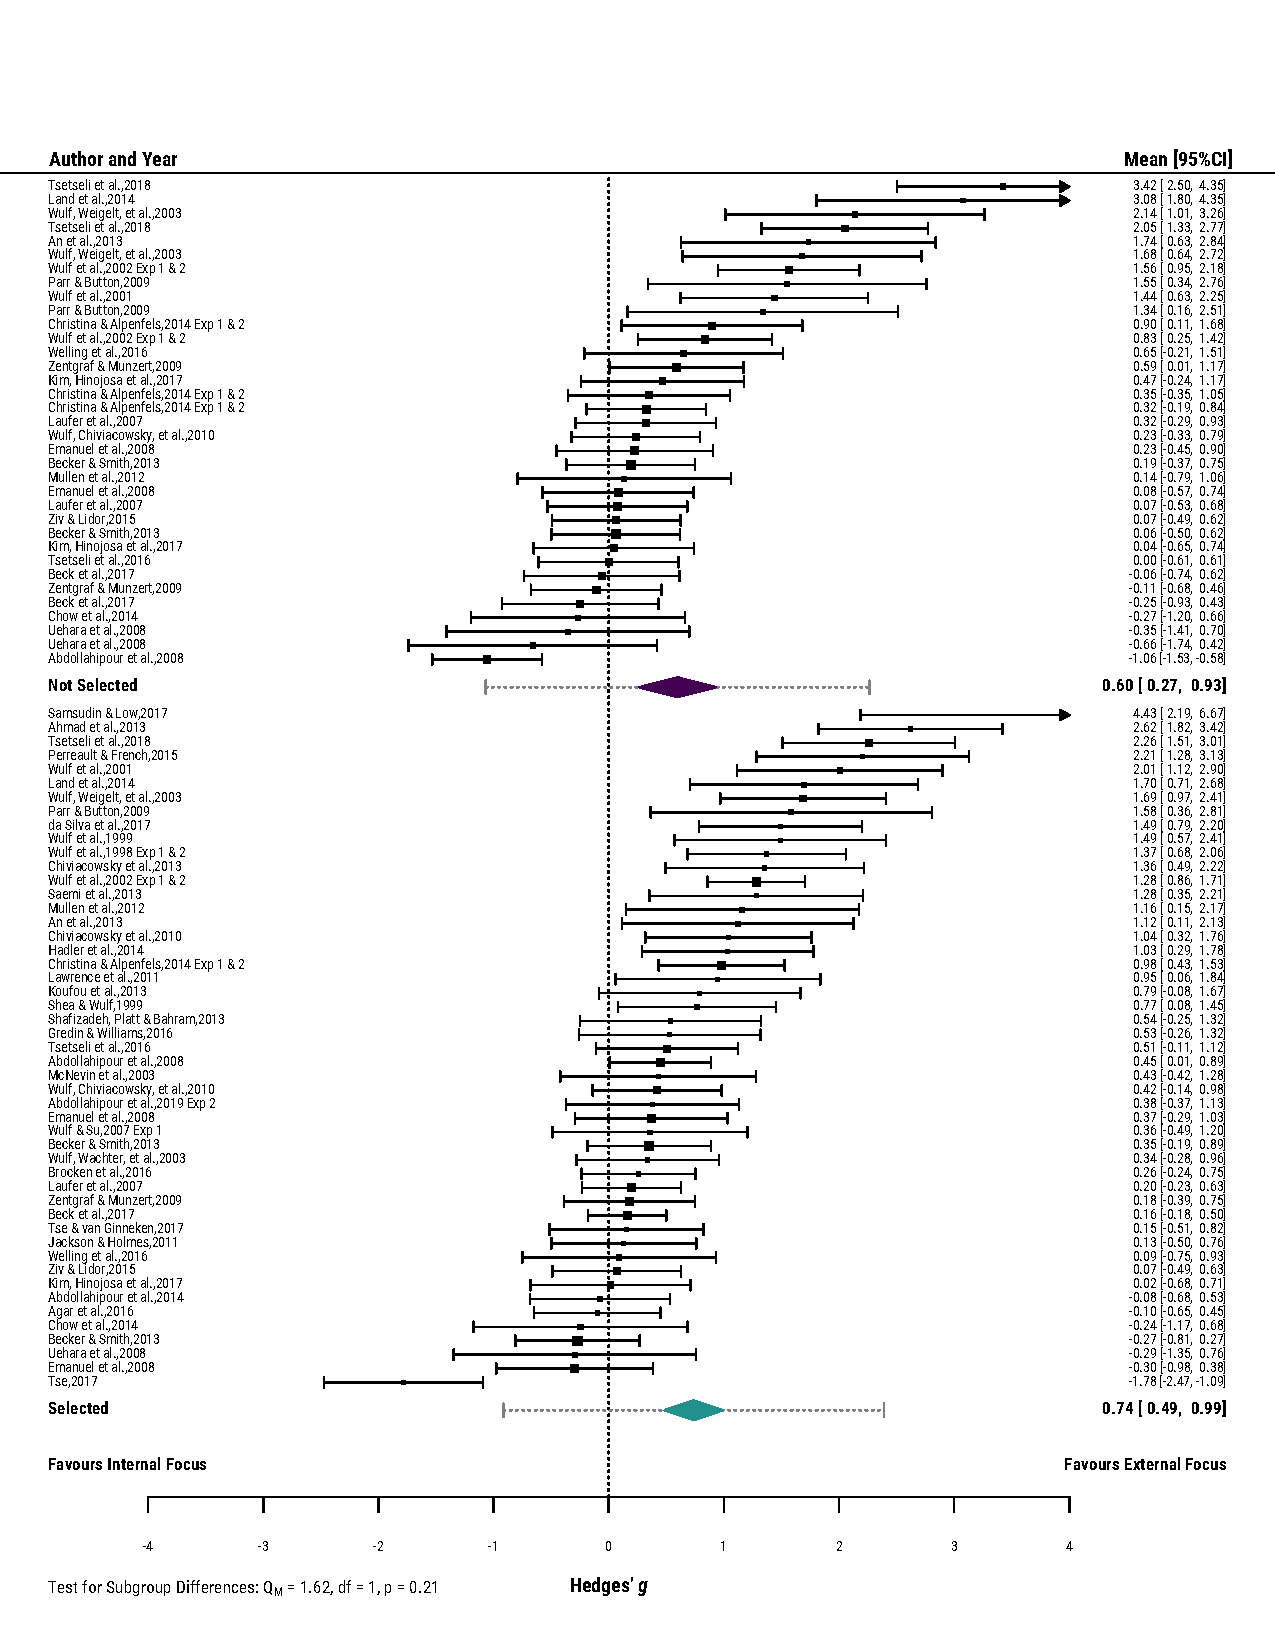
\includegraphics[height=0.715\textheight]{../../figs/fig2} 

}

\caption{\linespread{1.15}\selectfont \small \normalfont \textbf{Forest plot of retention outcomes separated by "selected" moderator.} Standardized mean difference (\emph{g}) and 95\% confidence intervals for each study included in the meta-analysis of retention outcomes. The green polygon represents the mean and 95\% confidence interval for outcomes that Chua et al. (2021) selected for analysis. The purple polygon represents the estimate for outcomes reported in the original experiments but were not selected by Chua et al. (2021). The error bars extending from both polygons reflect the 95\% prediction interval, illustrating the range of outcomes we would expect to observe in 95\% of studies randomly sampled from the same population of studies included in this analysis. The prediction intervals account for the substantial unexplained heterogeneity present in these data, showing that even without correcting for publication bias we would expect outcomes across the entire plausible range of effects.}\label{fig:fig2}
\end{figure}



\clearpage

\hypertarget{individual-model-fit}{%
\subsection{Individual model fit}\label{individual-model-fit}}

As implied by the results of each analysis, the best performing models overall assumed heterogeneity, publication bias, and zero effect (see Figure \ref{fig:fig3}). The best fitting publication bias models were the PET and PEESE funnel plot regression models, as well as the selection models that assumed directional hypotheses, particularly those that modeled censorship based on the direction of the point estimate. This pattern of findings suggests complex, results-based selection mechanisms linked to more than just statistical significance.

\clearpage

\begin{figure}

{\centering 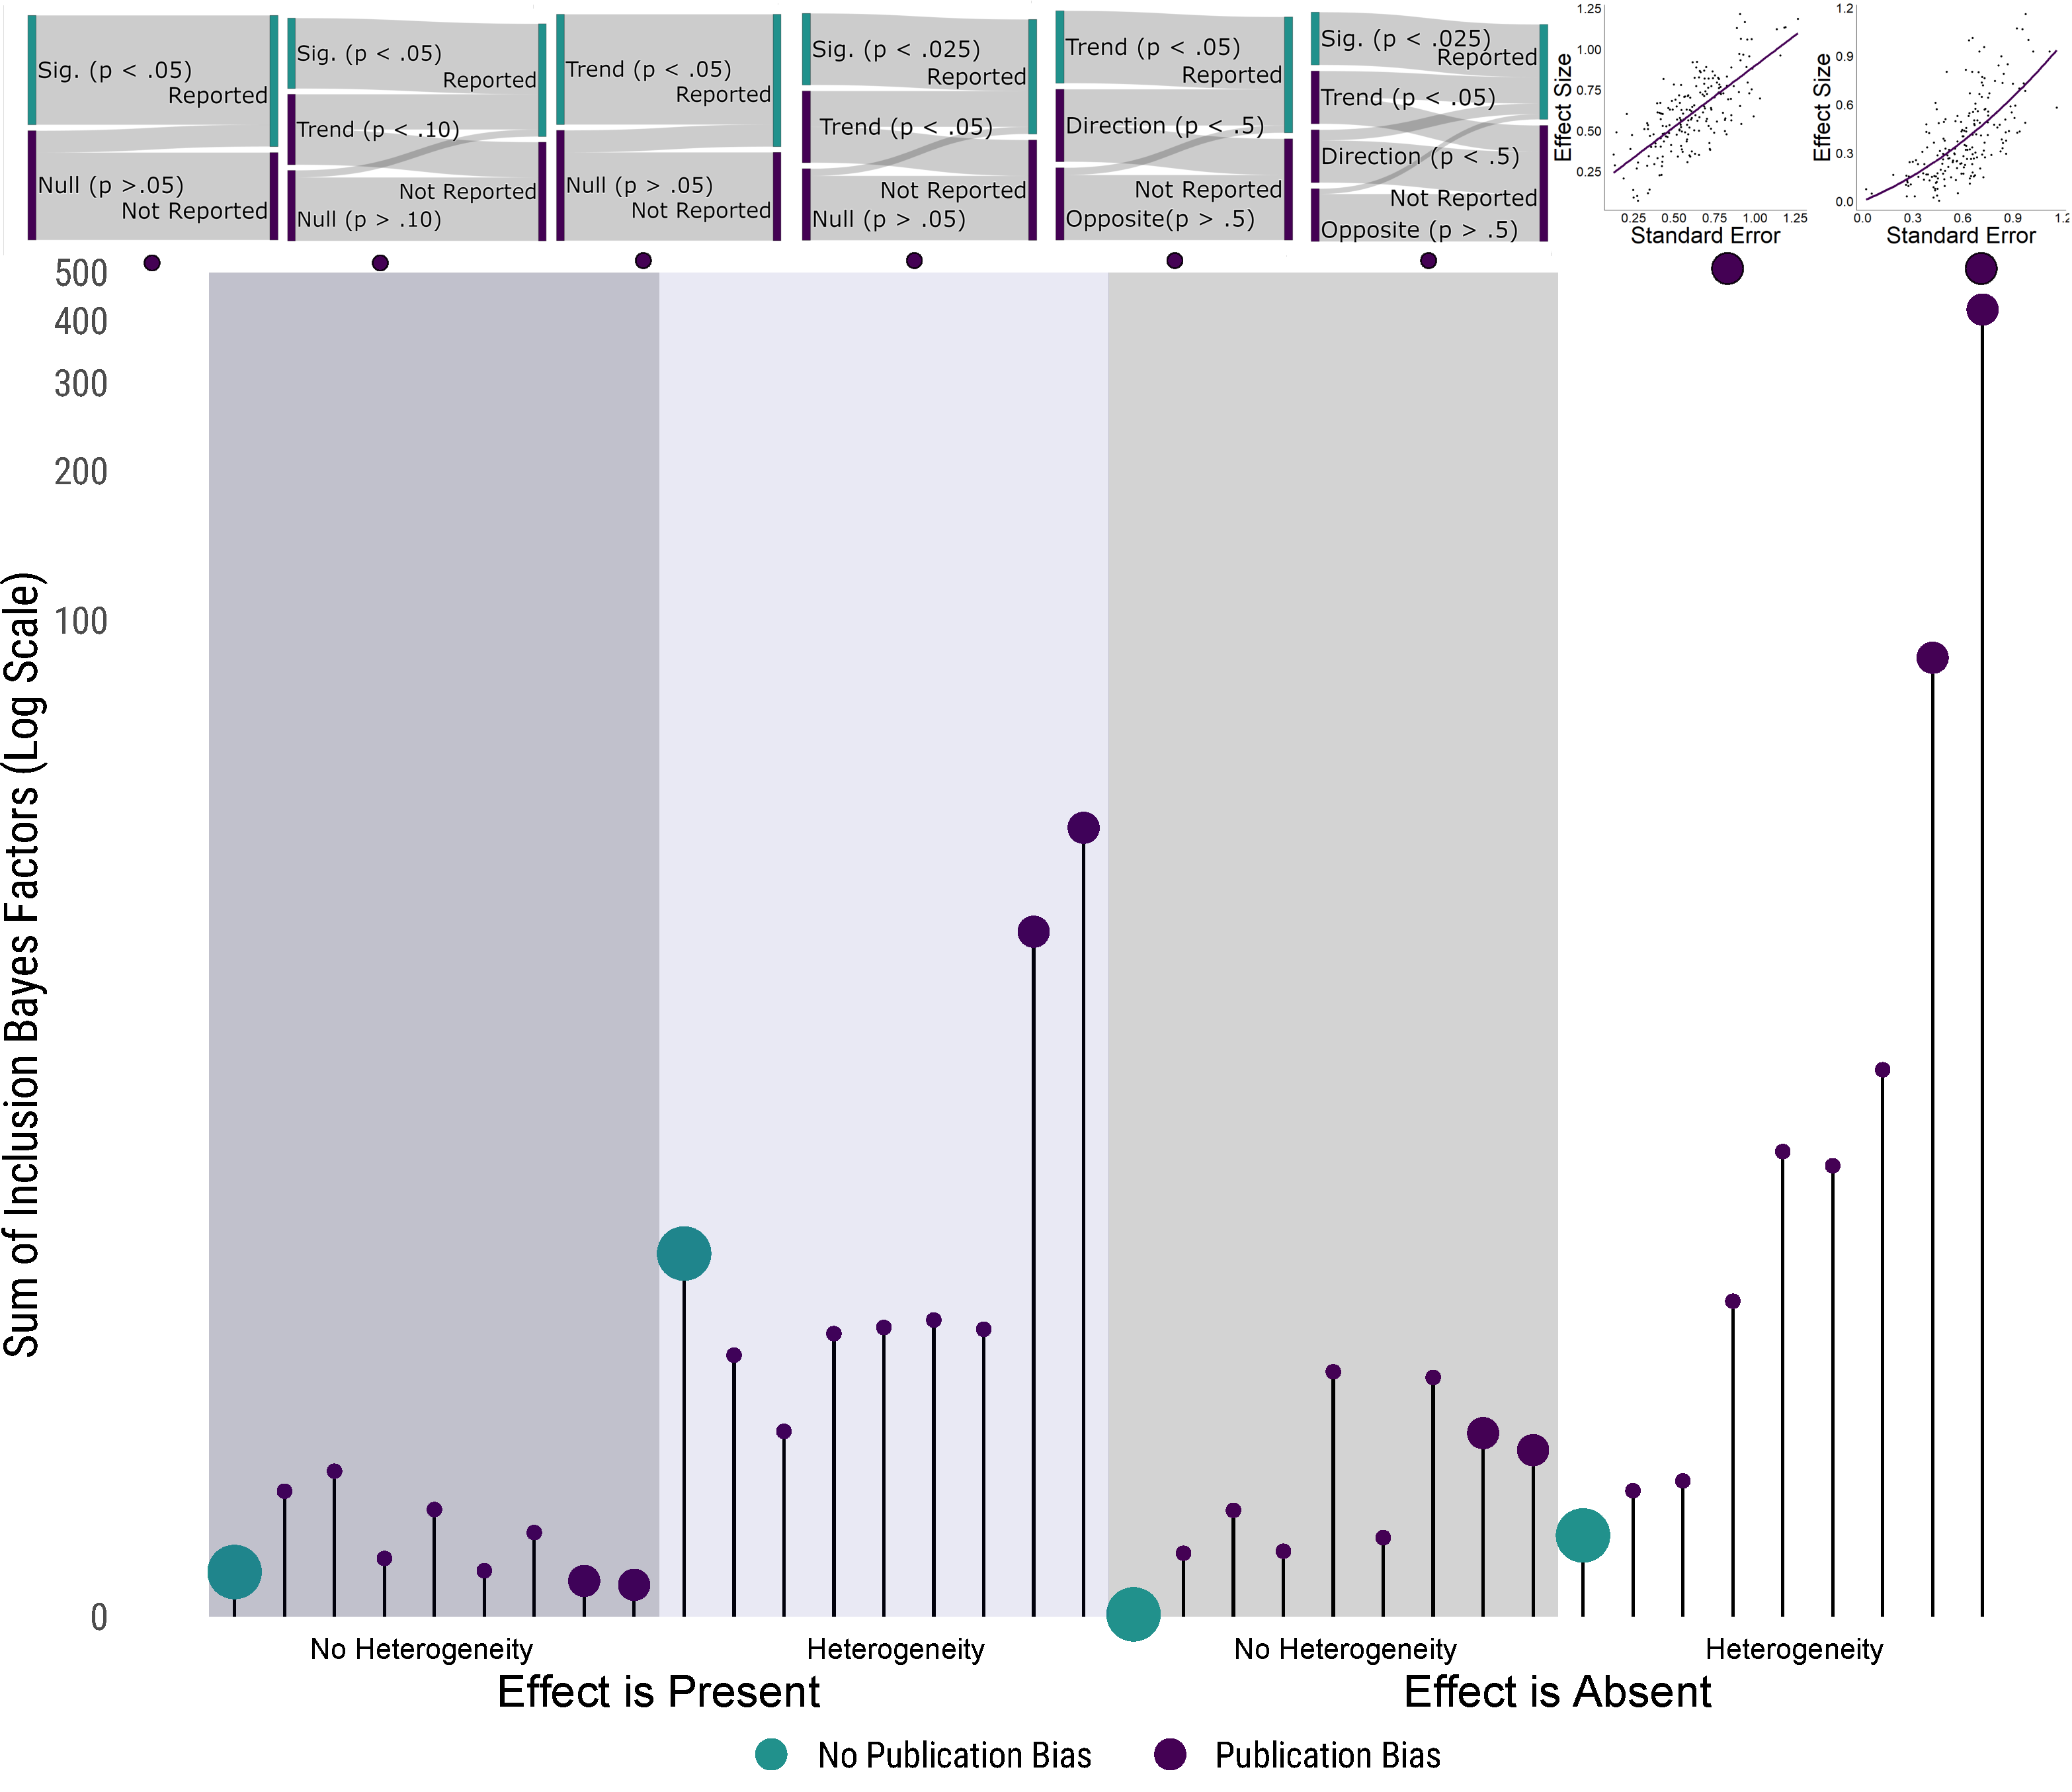
\includegraphics[width=0.99\linewidth]{../../figs/fig3} 

}

\caption{\linespread{1.15}\selectfont \small \normalfont \textbf{Total Inclusion Bayes Factor for each model relative to the ensemble, summed across each of the five analyses with and without outliers.} Higher Inclusion Bayes Factors indicate better agreement with the data than the average of the ensemble. The green circles represent naïve fixed and random effects models that assume no publication bias. The purple circles represent six selection models and two regression models, each modeling publication bias in a different way. A figure illustrating each of the publication bias models is displayed below the lollipop plot, shown in the same left-to-right order they follow in the plot above. The size of each circle reflects the prior probability assigned to the model (\emph{p} = .125 for naïve models, \emph{p} = .031 for regression models, and \emph{p} = .01 for selection models). The naïve and publication bias models were fit testing four scenarios: (a) an effect is present, no heterogeneity, (b) an effect is present, heterogeneity is present, (c) an effect is absent, no heterogeneity, and (d) an effect is absent, heterogeneity is present. The PEESE model, presented on the far right in each scenario, dominated the other models when assuming an effect is absent and heterogeneity is present. To better illustrate the performance of each model in the ensemble, Inclusion Bayes Factors are shown on a log scale on the \emph{y}-axis.}\label{fig:fig3}
\end{figure}



\clearpage

\hypertarget{discussion}{%
\section{Discussion}\label{discussion}}

We re-evaluated the evidence in support of an external focus benefit for learning, performance, muscular efficiency, and the distance effect. Seven previous meta-analyses have relied on the results of naïve random effects models that assume zero reporting bias in the primary estimates. However, it has become clear that such an assumption may not be appropriate for motor learning research (McKay et al., 2023; McKay, Yantha, et al., 2022). Each of the previous seven meta-analyses concluded that an external focus is superior to an internal focus. T. Kim et al. (2017) reported the benefits applied to balance learning, performance, and transfer. Hubert Makaruk et al. (2020) found the same for jump performance and Li et al. (2022) reported similar results for sprint performance. Grgic and colleagues reported external focus benefits for both muscular strength and endurance (Grgic et al., 2021; Grgic \& Mikulic, 2022). Nicklas et al. (2022) reported the advantage of an external focus over an internal focus applied to immediate performance in general. The most comprehensive of the meta-analyses, and the study whose data we reanalyzed, was conducted by Chua et al. (2021). They estimated small to moderate benefits for each specific effect and concluded that no amount of publication bias could attenuate the observed effects to zero.

Our results differ from previous meta-anayses as reporting bias was unaccounted for in their primary estimates. This is a serious limitation of the previous external focus meta-analyses as simulation studies have clearly demonstrated that random-effects result in large biases and high rates of false positives in the presence of publication-selection bias (Bartoš, Maier, Shanks, et al., 2023; Bom \& Rachinger, 2019; Stanley et al., 2017, 2022), which have been further supported when random-effects are compared with preregistered multilab replications (Kvarven et al., 2020). We therefore explicitly modeled bias and estimated trivially small effects in each analysis. While Chua et al. (2021) concluded that no amount of publication bias could reduce the effects to the null, our models suggest the data favor the null hypothesis for each analysis. If the only type of reporting bias in the literature is one-sided selection at \emph{p} = .05, then Chua and colleagues' conclusions were justified. However, if there were other considerations, such as sample size, trends, and direction of point estimates, the assumptions of their model were violated. Our analysis suggests this is the case for the focus of attention literature. Thus, similar to previous simulation studies our findings illustrate that reporting bias can cause random effects models to produce even large effect estimates when the true model is null. The random effects estimates reported by (Chua et al., 2021) ranged from small to large, while our corrected estimates range from essentially nil to trivial at best.

Although we observed somewhat larger estimates among effects selected by Chua et al. (2021) than among alternative outcomes that could have been selected, the difference was small and easily attributable to chance. The stronger signal for selection came from censorship prior to appearing in the published sample. Thus, the average reader of this literature would not have been inoculated against bias by having access to the complete results of each paper. The biasing influence of censorship would have already affected the sample of information readers could access.

These findings underscore uncertainty about external focus benefits. Adding to this uncertainty, we observed significant unexplained heterogeneity in effects. This heterogeneity could imply that focus of attention has a range of effects that depend on situational factors. If so, our results suggest that an internal focus may be superior to an external focus in nearly as many situations as the reverse. Alternatively, this heterogeneity may be due to methodological idiosyncrasies, unmodeled selection, or poor data curation at any level. As with censorship mechanisms, we have no way to know which potential sources of heterogeneity were at play.

Unfortunately, the present results add to a growing body of metascience questioning the extant support for the predictions in OPTIMAL theory (see McKay et al., 2023 for a recent meta-analysis on the other two pillars in the theory). In addition to predicting external focus benefits for learning and performance, OPTIMAL theory also predicts beneficial effects for autonomy and enhanced expectancies via similar underlying mechanisms (Wulf \& Lewthwaite, 2016). The primary corpus of evidence supporting motor learning benefits from autonomy is the self-controlled practice literature. Self-controlled practice involves asking learners to choose an aspect of their practice environment and the published literature suggests this will confer noticeable benefits to performance and learning (for a review see Ste-Marie, Carter, \& Yantha, 2020). However, like the external focus literature, the self-controlled practice research shows substantial evidence of reporting bias and more support for the null hypothesis (McKay, Yantha, et al., 2022). Approximately the same pattern emerges for the enhanced expectancies research (Bacelar et al., 2022). While the published literature appears to unequivocally demonstrate the predicted motor benefits of enhancing a learner's expectancy for success, accounting for reporting bias suggests uncertainty and heterogeneity (McKay et al., 2023). Taken together, this meta-evidence suggests the underlying mechanism common to all three factors of the tripartite OPTIMAL theory may be censorship. The mechanisms forwarded in OPTIMAL theory are made no less valid by this conclusion; it is the evidence rather than the theory that has been impugned by this body of work.\footnote{This conclusion also applies to other theories and perspectives (e.g., ecological dynamics) that have been forwarded based on the extant attentional focus literature to account for a supposed external focus advantage (e.g., Davids et al., 2003; Gottwald, Davies, \& Owen, 2023; Hommel et al., 2001; Prinz, 1990; Wulf \& Prinz, 2001).}

\hypertarget{limitations}{%
\subsection{Limitations}\label{limitations}}

The evidence in the review contains small sample sizes and small to moderate risk of bias according to Chua and colleagues (2021). None of the studies were preregistered. There were 20 studies missing due to insufficient information to calculate effect sizes in the original data set and another four missing effects from our extraction of secondary outcomes.

We did not explore whether manipulation checks verified that the instructed attentional focus was adopted during performance. OPTIMAL theory predicts that when learners focus on their intended effect on the environment, they facilitate goal-action coupling, benefiting learning and performance. Our analysis only investigated whether instructions or feedback impacted performance. Perhaps a missing moderator in our analysis was the extent to which focus instructions were followed in each experiment. We chose not to explore this possibility because there are no validated manipulation checks.

\hypertarget{recommendations-and-conclusions}{%
\subsection{Recommendations and conclusions}\label{recommendations-and-conclusions}}

The potential benefit of adopting an external focus of attention is among the most important contributions of academic motor learning research. It fits with numerous theoretical perspectives in the scientific literature and has been widely promoted in an array of applied settings, including sports, rehabilitation, and education. Our findings impugn the evidential basis for the superiority of an external focus of attention. However, rather than establishing nil or trivial benefits from focusing externally, uncertainty remains. The posteriors include interesting effects, there may be important moderators, and our estimates may have overcorrected for bias. We simply do not know if an external focus provides meaningful benefits to motor learning and performance or not. Moving forward, it will therefore be critical for researchers conducting meta-analyses in motor learning and related areas (e.g., psychology, neuroscience, sport and exercise science) to adopt the use of leverage statistics as the default approach for identifying outliers (see Deeks, Higgins, Altman, \& Cochrane Statistical Methods Group, 2023; Viechtbauer \& Cheung, 2010 for discussions).

Building knowledge about external focus effects can be accelerated by adoption of the Registered Report publication format (Chambers, 2019). Registered Reports prevent publication bias (Scheel, Schijen, \& Lakens, 2021), and when they include preregistration of analysis plans, they prevent \emph{p}-hacking (Simmons, Nelson, \& Simonsohn, 2011) and HARKing (Kerr, 1998) as well. Limited resources may prevent individual laboratories from collecting sufficient sample sizes for a well-powered Registered Report, so researchers are encouraged to collaborate extensively to achieve the sample sizes necessary to make progress.

\newpage

\hypertarget{references}{%
\section{References}\label{references}}

References marked with an asterisk (*) indicate studies included in the meta-analysis.

\vspace{2ex}

\hypertarget{refs}{}
\begin{CSLReferences}{1}{0}
\leavevmode\vadjust pre{\hypertarget{ref-abdollahipour2008-meta}{}}%
\textsuperscript{*} Abdollahipour, R., Bahram, A., Shafizadeh, M., \& Khalaji, H. (2008). The effects of attentional focus strategies on the performance and learning of soccer-dribbling task in children and adolescences. \emph{Journal of Movement Sciences and Sports}, \emph{1}, 83--92.

\leavevmode\vadjust pre{\hypertarget{ref-abdollahipour2020-meta}{}}%
\textsuperscript{*} Abdollahipour, Reza, Land, W. M., Cereser, A., \& Chiviacowsky, S. (2020). External relative to internal attentional focus enhances motor performance and learning in visually impaired individuals. \emph{Disability and Rehabilitation}, \emph{42}(18), 2621--2630.

\leavevmode\vadjust pre{\hypertarget{ref-abdollahipour2017-meta}{}}%
\textsuperscript{*} Abdollahipour, Reza, \& Psotta, R. (2017). Is an external focus of attention more beneficial than an internal focus to ball catching in children? \emph{Kinesiology}, \emph{49}(2.), 235--241.

\leavevmode\vadjust pre{\hypertarget{ref-abdollahipour2016-meta}{}}%
\textsuperscript{*} Abdollahipour, Reza, Psotta, R., \& Land, W. M. (2016). The influence of attentional focus instructions and vision on jump height performance. \emph{Research Quarterly for Exercise and Sport}, \emph{87}(4), 408--413.

\leavevmode\vadjust pre{\hypertarget{ref-abdollahipour2014-meta}{}}%
\textsuperscript{*} Abdollahipour, Reza, Psotta, R., Palomo Nieto, M., Rouzbahani, M., Nikdast, H., \& Bahram, A. (2014). Effects of attentional focus instructions on the learning of a target task: A moderation role of visual feedback. \emph{Kinesiology}, \emph{46}(2), 210--217.

\leavevmode\vadjust pre{\hypertarget{ref-abdollahipour2015-meta}{}}%
\textsuperscript{*} Abdollahipour, Reza, Wulf, G., Psotta, R., \& Palomo Nieto, M. (2015). Performance of gymnastics skill benefits from an external focus of attention. \emph{Journal of Sports Sciences}, \emph{33}(17), 1807--1813.

\leavevmode\vadjust pre{\hypertarget{ref-agar2016-meta}{}}%
\textsuperscript{*} Agar, C., Humphries, C. A., Naquin, M., Hebert, E., \& Wood, R. (2016). Does varying attentional focus affect skill acquisition in children? A comparison of internal and external focus instructions and feedback. \emph{Physical Educator}, \emph{73}(4), 639--651.

\leavevmode\vadjust pre{\hypertarget{ref-ahmad2013-meta}{}}%
\textsuperscript{*} Ahmad, A., Fadhil, A., \& Shakir, H. (2013). The effects of external and internal focus of attention on upper volleyball serve. \emph{International Journal of Advanced Sport Sciences Research}, \emph{1}, 155--163.

\leavevmode\vadjust pre{\hypertarget{ref-appelbaum2018}{}}%
Appelbaum, M., Cooper, H., Kline, R. B., Mayo-Wilson, E., Nezu, A. M., \& Rao, S. M. (2018). Journal article reporting standards for quantitative research in psychology: The APA publications and communications board task force report. \emph{American Psychologist}, \emph{73}(1), 3.

\leavevmode\vadjust pre{\hypertarget{ref-asadi2015-meta}{}}%
\textsuperscript{*} Asadi, A., Abdoli, B., Farsi, A., \& Saemi, E. (2015). Effect of various attentional focus instructions on novice javelin throwing skill performance. \emph{Medicina Dello Sport}, \emph{68}(1), 99--107.

\leavevmode\vadjust pre{\hypertarget{ref-ashraf2017-meta}{}}%
\textsuperscript{*} Ashraf, R., Aghdasi, M. T., \& Sayyah, M. (2017). The effect of attentional focus strategies on children performance and their EMG activities in maximum a force production task. \emph{Turkish Journal of Kinesiology}, \emph{3}(2), 26--30.

\leavevmode\vadjust pre{\hypertarget{ref-R-papaja}{}}%
Aust, F., \& Barth, M. (2020). \emph{{papaja}: {Prepare} reproducible {APA} journal articles with {R Markdown}}. Retrieved from \url{https://github.com/crsh/papaja}

\leavevmode\vadjust pre{\hypertarget{ref-bacelar2022b}{}}%
Bacelar, M. F. B., Parma, J. O., Murrah, W. M., \& Miller, M. W. (2022). Meta-analyzing enhanced expectancies on motor learning: Positive effects but methodological concerns. \emph{International Review of Sport and Exercise Psychology}, \emph{0}(0), 1--30. \url{https://doi.org/10.1080/1750984X.2022.2042839}

\leavevmode\vadjust pre{\hypertarget{ref-R-tinylabels}{}}%
Barth, M. (2022). \emph{{tinylabels}: Lightweight variable labels}. Retrieved from \url{https://cran.r-project.org/package=tinylabels}

\leavevmode\vadjust pre{\hypertarget{ref-R-RoBMA}{}}%
Bartoš, F., \& Maier, M. (2020). \emph{RoBMA: An r package for robust bayesian meta-analyses}. Retrieved from \url{https://CRAN.R-project.org/package=RoBMA}

\leavevmode\vadjust pre{\hypertarget{ref-bartos2023a}{}}%
Bartoš, F., Maier, M., Shanks, D. R., Stanley, T., Sladekova, M., \& Wagenmakers, E.-J. (2023). Meta-analyses in psychology often overestimate evidence for and size of effects. \emph{Royal Society Open Science}, \emph{10}(7), 230224.

\leavevmode\vadjust pre{\hypertarget{ref-bartos2023}{}}%
Bartoš, F., Maier, M., Wagenmakers, E.-J., Doucouliagos, H., \& Stanley, T. D. (2023). Robust {Bayesian} meta-analysis: {Model-averaging} across complementary publication bias adjustment methods. \emph{Research Synthesis Methods}, \emph{14}(1), 99--116. \url{https://doi.org/10.1002/jrsm.1594}

\leavevmode\vadjust pre{\hypertarget{ref-beck2017-meta}{}}%
\textsuperscript{*} Beck, E. N., \& Almeida, Q. J. (2017). Dopa-responsive balance changes depend on use of internal versus external attentional focus in parkinson disease. \emph{Physical Therapy}, \emph{97}(2), 208--216.

\leavevmode\vadjust pre{\hypertarget{ref-beck2018can}{}}%
\textsuperscript{*} Beck, E. N., Intzandt, B. N., \& Almeida, Q. J. (2018). Can dual task walking improve in parkinson's disease after external focus of attention exercise? A single blind randomized controlled trial. \emph{Neurorehabilitation and Neural Repair}, \emph{32}(1), 18--33.

\leavevmode\vadjust pre{\hypertarget{ref-becker2013-meta}{}}%
\textsuperscript{*} Becker, K., \& Smith, P. J. (2013). Age, task complexity, and sex as potential moderators of attentional focus effects. \emph{Perceptual and Motor Skills}, \emph{117}(1), 130--144.

\leavevmode\vadjust pre{\hypertarget{ref-bernier2016}{}}%
Bernier, M., Trottier, C., Thienot, E., \& Fournier, J. (2016). An investigation of attentional foci and their temporal patterns: A naturalistic study in expert figure skaters. \emph{The Sport Psychologist}, \emph{30}(3), 256--266.

\leavevmode\vadjust pre{\hypertarget{ref-bom2019}{}}%
Bom, P. R., \& Rachinger, H. (2019). A kinked meta-regression model for publication bias correction. \emph{Research Synthesis Methods}, \emph{10}(4), 497--514.

\leavevmode\vadjust pre{\hypertarget{ref-R-PublicationBias}{}}%
Braginsky, M., Mathur, M., \& VanderWeele, T. J. (2023). \emph{PublicationBias: Sensitivity analysis for publication bias in meta-analyses}. Retrieved from \url{https://CRAN.R-project.org/package=PublicationBias}

\leavevmode\vadjust pre{\hypertarget{ref-brick2014}{}}%
Brick, N., MacIntyre, T., \& Campbell, M. (2014). Attentional focus in endurance activity: New paradigms and future directions. \emph{International Review of Sport and Exercise Psychology}, \emph{7}(1), 106--134.

\leavevmode\vadjust pre{\hypertarget{ref-brocken2016-meta}{}}%
\textsuperscript{*} Brocken, J., Kal, E., \& Van der Kamp, J. (2016). Focus of attention in children's motor learning: Examining the role of age and working memory. \emph{Journal of Motor Behavior}, \emph{48}(6), 527--534.

\leavevmode\vadjust pre{\hypertarget{ref-canning2005}{}}%
Canning, C. G. (2005). The effect of directing attention during walking under dual-task conditions in parkinson's disease. \emph{Parkinsonism \& Related Disorders}, \emph{11}(2), 95--99.

\leavevmode\vadjust pre{\hypertarget{ref-carter2015}{}}%
Carter, E. C., Kofler, L. M., Forster, D. E., \& McCullough, M. E. (2015). A series of meta-analytic tests of the depletion effect: {Self-control} does not seem to rely on a limited resource. \emph{Journal of Experimental Psychology: General}, \emph{144}(4), 796--815. \url{https://doi.org/10.1037/xge0000083}

\leavevmode\vadjust pre{\hypertarget{ref-carter2019}{}}%
Carter, E. C., Schönbrodt, F. D., Gervais, W. M., \& Hilgard, J. (2019). Correcting for {Bias} in {Psychology}: {A Comparison} of {Meta-Analytic Methods}. \emph{Advances in Methods and Practices in Psychological Science}, \emph{2}(2), 115--144. \url{https://doi.org/10.1177/2515245919847196}

\leavevmode\vadjust pre{\hypertarget{ref-chambers2019}{}}%
Chambers, C. (2019). What's next for {Registered Reports}? \emph{Nature}, \emph{573}(7773), 187--189.

\leavevmode\vadjust pre{\hypertarget{ref-R-extrafont}{}}%
Chang, W. (2023). \emph{Extrafont: Tools for using fonts}. Retrieved from \url{https://CRAN.R-project.org/package=extrafont}

\leavevmode\vadjust pre{\hypertarget{ref-chiviacowsky2013-meta}{}}%
\textsuperscript{*} Chiviacowsky, S., Wulf, G., \& Ávila, L. (2013). An external focus of attention enhances motor learning in children with intellectual disabilities. \emph{Journal of Intellectual Disability Research}, \emph{57}(7), 627--634.

\leavevmode\vadjust pre{\hypertarget{ref-chiviacowsky2010-meta}{}}%
\textsuperscript{*} Chiviacowsky, Suzete, Wulf, G., \& Wally, R. (2010). An external focus of attention enhances balance learning in older adults. \emph{Gait \& Posture}, \emph{32}(4), 572--575.

\leavevmode\vadjust pre{\hypertarget{ref-chow2014-meta}{}}%
\textsuperscript{*} Chow, J. Y., Woo, M. T., \& Koh, M. (2014). Effects of external and internal attention focus training on foot-strike patterns in running. \emph{International Journal of Sports Science \& Coaching}, \emph{9}(2), 307--320.

\leavevmode\vadjust pre{\hypertarget{ref-christina2014-meta}{}}%
\textsuperscript{*} Christina, B., \& Alpenfels, E. (2014). Influence of attentional focus on learning a swing path change. \emph{International Journal of Golf Science}, \emph{3}(1), 35--49.

\leavevmode\vadjust pre{\hypertarget{ref-chua2021}{}}%
Chua, L.-K., Jimenez-Diaz, J., Lewthwaite, R., Kim, T., \& Wulf, G. (2021). Superiority of external attentional focus for motor performance and learning: {Systematic} reviews and meta-analyses. \emph{Psychological Bulletin}, \emph{147}, 618--645. \url{https://doi.org/10.1037/bul0000335}

\leavevmode\vadjust pre{\hypertarget{ref-coker2016-meta}{}}%
\textsuperscript{*} Coker, C. (2016). Optimizing external focus of attention instructions: The role of attainability. \emph{Journal of Motor Learning and Development}, \emph{4}(1), 116--125.

\leavevmode\vadjust pre{\hypertarget{ref-coker2018-meta}{}}%
\textsuperscript{*} Coker, C. (2018). Kinematic effects of varying adolescents' attentional instructions for standing long jump. \emph{Perceptual and Motor Skills}, \emph{125}(6), 1093--1102.

\leavevmode\vadjust pre{\hypertarget{ref-collins2016}{}}%
Collins, D., Carson, H. J., \& Toner, J. (2016). Letter to the editor concerning the article {``performance of gymnastics skill benefits from an external focus of attention''} by abdollahipour, wulf, psotta \& nieto (2015). \emph{Journal of Sports Sciences}, \emph{34}(13), 1288--1292.

\leavevmode\vadjust pre{\hypertarget{ref-davids2003}{}}%
Davids, K., Araújo, D., Shuttleworth, R., \& Button, C. (2003). Acquiring skill in sport: {A} constraints-led perspective. \emph{International Journal of Computer Science in Sport}.

\leavevmode\vadjust pre{\hypertarget{ref-de2017-meta}{}}%
\textsuperscript{*} de Melker Worms, J. L., Stins, J. F., Wegen, E. E. van, Loram, I. D., \& Beek, P. J. (2017). Influence of focus of attention, reinvestment and fall history on elderly gait stability. \emph{Physiological Reports}, \emph{5}(1), e13061.

\leavevmode\vadjust pre{\hypertarget{ref-R-faux}{}}%
DeBruine, L. (2023). \emph{Faux: Simulation for factorial designs}. Zenodo. \url{https://doi.org/10.5281/zenodo.2669586}

\leavevmode\vadjust pre{\hypertarget{ref-deeks2023}{}}%
Deeks, J. J., Higgins, J. P., Altman, D. G., \& Cochrane Statistical Methods Group, on behalf of the. (2023). Analysing data and undertaking meta-analyses. In J. P. T. Higgins, J. Thomas, J. Chandler, M. Cumpston, T. Li, M. J. Page, \& V. A. Welch (Eds.), \emph{Cochrane handbook for systematic reviews of interventions} (Version 6.4). Wiley Online Library.

\leavevmode\vadjust pre{\hypertarget{ref-diekfuss2018-meta}{}}%
\textsuperscript{*} Diekfuss, J. A., Janssen, J. A., Slutsky, A. B., Berry, N. T., Etnier, J. L., Wideman, L., \& Raisbeck, L. D. (2018). An external focus of attention is effective for balance control when sleep-deprived. \emph{International Journal of Exercise Science}, \emph{11}(5), 84.

\leavevmode\vadjust pre{\hypertarget{ref-ducharme2015-meta}{}}%
\textsuperscript{*} Ducharme, S. W., \& Wu, W. F. (2015). An external focus of attention improves stability after a perturbation during a dynamic balance task. \emph{Journal of Motor Learning and Development}, \emph{3}(2), 74--90.

\leavevmode\vadjust pre{\hypertarget{ref-ducharme2016-meta}{}}%
\textsuperscript{*} Ducharme, S. W., Wu, W. F., Lim, K., Porter, J. M., \& Geraldo, F. (2016). Standing long jump performance with an external focus of attention is improved as a result of a more effective projection angle. \emph{The Journal of Strength \& Conditioning Research}, \emph{30}(1), 276--281.

\leavevmode\vadjust pre{\hypertarget{ref-duke2011-meta}{}}%
\textsuperscript{*} Duke, R. A., Cash, C. D., \& Allen, S. E. (2011). Focus of attention affects performance of motor skills in music. \emph{Journal of Research in Music Education}, \emph{59}(1), 44--55.

\leavevmode\vadjust pre{\hypertarget{ref-durham2014-meta}{}}%
\textsuperscript{*} Durham, K., Sackley, C., Wright, C., Wing, A., Edwards, M., \& Van Vliet, P. (2014). Attentional focus of feedback for improving performance of reach-to-grasp after stroke: A randomised crossover study. \emph{Physiotherapy}, \emph{100}(2), 108--115.

\leavevmode\vadjust pre{\hypertarget{ref-emanuel2008-meta}{}}%
\textsuperscript{*} Emanuel, M., Jarus, T., \& Bart, O. (2008). Effect of focus of attention and age on motor acquisition, retention, and transfer: A randomized trial. \emph{Physical Therapy}, \emph{88}(2), 251--260.

\leavevmode\vadjust pre{\hypertarget{ref-fasoli2002-meta}{}}%
\textsuperscript{*} Fasoli, S. E., Trombly, C. A., Tickle-Degnen, L., \& Verfaellie, M. H. (2002). Effect of instructions on functional reach in persons with and without cerebrovascular accident. \emph{The American Journal of Occupational Therapy}, \emph{56}(4), 380--390.

\leavevmode\vadjust pre{\hypertarget{ref-R-daff}{}}%
Fitzpatrick, P., de Jonge, E., \& Warnes, G. R. (2019). \emph{Daff: Diff, patch and merge for data.frames}. Retrieved from \url{https://CRAN.R-project.org/package=daff}

\leavevmode\vadjust pre{\hypertarget{ref-flores2015-meta}{}}%
\textsuperscript{*} Flores, F. S., Schild, J. F. G., \& Chiviacowsky, S. (2015). Benefits of external focus instructions on the learning of a balance task in children of different ages. \emph{International Journal of Sport Psychology}, \emph{46}(4), 311--320.

\leavevmode\vadjust pre{\hypertarget{ref-freudenheim2010-meta}{}}%
\textsuperscript{*} Freudenheim, A. M., Wulf, G., Madureira, F., Pasetto, S. C., \& Corrěa, U. C. (2010). An external focus of attention results in greater swimming speed. \emph{International Journal of Sports Science \& Coaching}, \emph{5}(4), 533--542.

\leavevmode\vadjust pre{\hypertarget{ref-R-stringi}{}}%
Gagolewski, M. (2022). {stringi}: {F}ast and portable character string processing in {R}. \emph{Journal of Statistical Software}, \emph{103}(2), 1--59. \url{https://doi.org/10.18637/jss.v103.i02}

\leavevmode\vadjust pre{\hypertarget{ref-gottwald2023}{}}%
Gottwald, V., Davies, M., \& Owen, R. (2023). Every story has two sides: {Evaluating} information processing and ecological dynamics perspectives of focus of attention in skill acquisition. \emph{Frontiers in Sports and Active Living}, \emph{5}, 167.

\leavevmode\vadjust pre{\hypertarget{ref-gredin2016-meta}{}}%
\textsuperscript{*} Gredin, V., \& Williams, A. M. (2016). The relative effectiveness of various instructional approaches during the performance and learning of motor skills. \emph{Journal of Motor Behavior}, \emph{48}(1), 86--97.

\leavevmode\vadjust pre{\hypertarget{ref-greig2014-meta}{}}%
\textsuperscript{*} Greig, M., \& Marchant, D. (2014). Speed dependant influence of attentional focusing instructions on force production and muscular activity during isokinetic elbow flexions. \emph{Human Movement Science}, \emph{33}, 135--148.

\leavevmode\vadjust pre{\hypertarget{ref-grgic2021}{}}%
Grgic, J., Mikulic, I., \& Mikulic, P. (2021). Acute and long-term effects of attentional focus strategies on muscular strength: {A} meta-analysis. \emph{Sports}, \emph{9}(11, 11), 153. \url{https://doi.org/10.3390/sports9110153}

\leavevmode\vadjust pre{\hypertarget{ref-grgic2022}{}}%
Grgic, J., \& Mikulic, P. (2022). Effects of attentional focus on muscular endurance: {A} meta-analysis. \emph{International Journal of Environmental Research and Public Health}, \emph{19}(1, 1), 89. \url{https://doi.org/10.3390/ijerph19010089}

\leavevmode\vadjust pre{\hypertarget{ref-hadler2014-meta}{}}%
\textsuperscript{*} Hadler, R., Chiviacowsky, S., Wulf, G., \& Schild, J. F. G. (2014). Children's learning of tennis skills is facilitated by external focus instructions. \emph{Motriz: Revista de Educa{ç}{ã}o F{ı́}sica}, \emph{20}, 418--422.

\leavevmode\vadjust pre{\hypertarget{ref-halperin2017-meta}{}}%
\textsuperscript{*} Halperin, I., Chapman, D. W., Martin, D. T., \& Abbiss, C. (2017). The effects of attentional focus instructions on punching velocity and impact forces among trained combat athletes. \emph{Journal of Sports Sciences}, \emph{35}(5), 500--507.

\leavevmode\vadjust pre{\hypertarget{ref-halperin2016-meta}{}}%
\textsuperscript{*} Halperin, I., Hughes, S., Panchuk, D., Abbiss, C., \& Chapman, D. W. (2016). The effects of either a mirror, internal or external focus instructions on single and multi-joint tasks. \emph{PLoS One}, \emph{11}(11), e0166799.

\leavevmode\vadjust pre{\hypertarget{ref-halperin2016b-meta}{}}%
\textsuperscript{*} Halperin, I., Williams, K. J., Martin, D. T., \& Chapman, D. W. (2016). The effects of attentional focusing instructions on force production during the isometric midthigh pull. \emph{The Journal of Strength \& Conditioning Research}, \emph{30}(4), 919--923.

\leavevmode\vadjust pre{\hypertarget{ref-hebert2017-meta}{}}%
\textsuperscript{*} Hebert, E. P., \& Williams, B. M. (2017). Effects of three types of attentional focus on standing long jump performance. \emph{Journal of Sport Behavior}, \emph{40}(2), 156--170.

\leavevmode\vadjust pre{\hypertarget{ref-hill2017-meta}{}}%
\textsuperscript{*} Hill, A., Schücker, L., Hagemann, N., \& Strauß, B. (2017). Further evidence for an external focus of attention in running: Looking at specific focus instructions and individual differences. \emph{Journal of Sport and Exercise Psychology}, \emph{39}(5), 352--365.

\leavevmode\vadjust pre{\hypertarget{ref-hommel2001}{}}%
Hommel, B., Müsseler, J., Aschersleben, G., \& Prinz, W. (2001). The {Theory} of {Event Coding} ({TEC}): {A} framework for perception and action planning. \emph{Behavioral and Brain Sciences}, \emph{24}(5), 849--878. \url{https://doi.org/10.1017/S0140525X01000103}

\leavevmode\vadjust pre{\hypertarget{ref-hosseiny2014c-meta}{}}%
\textsuperscript{*} Hosseiny, S. H., Ghasemi, A., \& Shakeri, N. (2014). Comparing the effects of internal, external and prefer focus of attention on the elite shooters' performance. \emph{Advances in Environmental Biology}, \emph{8}(5), 1245--1250.

\leavevmode\vadjust pre{\hypertarget{ref-huang2014-meta}{}}%
\textsuperscript{*} Huang, C.-Y., Zhao, C.-G., \& Hwang, S. (2014). Neural basis of postural focus effect on concurrent postural and motor tasks: Phase-locked electroencephalogram responses. \emph{Behavioural Brain Research}, \emph{274}, 95--107.

\leavevmode\vadjust pre{\hypertarget{ref-hussien2023a}{}}%
Hussien, J., Gignac, L., Shearer, L., \& Ste-Marie, D. M. (2023a). The path to translating focus of attention research into {Canadian} physiotherapy, {Part} 2: {Physiotherapist} interviews reveal impacting factors and barriers to focus of attention use. \emph{Journal of Motor Learning and Development}, \emph{1}(aop), 1--21. \url{https://doi.org/10.1123/jmld.2022-0053}

\leavevmode\vadjust pre{\hypertarget{ref-hussien2023b}{}}%
Hussien, J., Gignac, L., Shearer, L., \& Ste-Marie, D. M. (2023b). The path to translating focus of attention research into {Canadian} physiotherapy, {Part} 3: {Designing} a workshop through consultation with physiotherapists and focus of attention researchers. \emph{Journal of Motor Learning and Development}, \emph{1}(aop), 1--16. \url{https://doi.org/10.1123/jmld.2022-0067}

\leavevmode\vadjust pre{\hypertarget{ref-hussien2023}{}}%
Hussien, J., \& Ste-Marie, D. M. (2023). The path to translating focus of attention research into {Canadian} physiotherapy, {Part} 1: {Physiotherapists}' self-reported focus of attention use via a study-specific questionnaire. \emph{Journal of Motor Learning and Development}, \emph{11}(1), 86--99. \url{https://doi.org/10.1123/jmld.2022-0052}

\leavevmode\vadjust pre{\hypertarget{ref-R-gt}{}}%
Iannone, R., Cheng, J., Schloerke, B., Hughes, E., Lauer, A., \& Seo, J. (2023). \emph{Gt: Easily create presentation-ready display tables}. Retrieved from \url{https://CRAN.R-project.org/package=gt}

\leavevmode\vadjust pre{\hypertarget{ref-ille2013-meta}{}}%
\textsuperscript{*} Ille, A., Selin, I., Do, M.-C., \& Thon, B. (2013). Attentional focus effects on sprint start performance as a function of skill level. \emph{Journal of Sports Sciences}, \emph{31}(15), 1705--1712.

\leavevmode\vadjust pre{\hypertarget{ref-jackson2011-meta}{}}%
\textsuperscript{*} Jackson, B. H., \& Holmes, A. M. (2011). The effects of focus of attention and task objective consistency on learning a balancing task. \emph{Research Quarterly for Exercise and Sport}, \emph{82}(3), 574.

\leavevmode\vadjust pre{\hypertarget{ref-jazaeri2018-meta}{}}%
\textsuperscript{*} Jazaeri, S. Z., Azad, A., Mehdizadeh, H., Habibi, S. A., Mandehgary Najafabadi, M., Saberi, Z. S., et al.others. (2018). The effects of anxiety and external attentional focus on postural control in patients with parkinson's disease. \emph{PLoS One}, \emph{13}(2), e0192168.

\leavevmode\vadjust pre{\hypertarget{ref-johnson2023}{}}%
Johnson, L., Burridge, J., Ewings, S., Westcott, E., Gayton, M., \& Demain, S. (2023). Principles into practice: {An} observational study of physiotherapists use of motor learning principles in stroke rehabilitation. \emph{Physiotherapy}, \emph{118}, 20--30. \url{https://doi.org/10.1016/j.physio.2022.06.002}

\leavevmode\vadjust pre{\hypertarget{ref-kal2013-meta}{}}%
\textsuperscript{*} Kal, E., Van der Kamp, J., \& Houdijk, H. (2013). External attentional focus enhances movement automatization: A comprehensive test of the constrained action hypothesis. \emph{Human Movement Science}, \emph{32}(4), 527--539.

\leavevmode\vadjust pre{\hypertarget{ref-kalkhoran2014-meta}{}}%
\textsuperscript{*} Kalkhoran, J., Shariati, A., et al. (2014). The effect of attentional-focus instruction on peripheral transfer from dominant hand to non-dominant hand and vice versa in basketball dribbling. \emph{Pamukkale Journal of Sport Sciences}, \emph{5}(2).

\leavevmode\vadjust pre{\hypertarget{ref-R-ggdist}{}}%
Kay, M. (2023). \emph{{ggdist}: Visualizations of distributions and uncertainty}. \url{https://doi.org/10.5281/zenodo.3879620}

\leavevmode\vadjust pre{\hypertarget{ref-kearney2015-meta}{}}%
\textsuperscript{*} Kearney, P. E. (2015). A distal focus of attention leads to superior performance on a golf putting task. \emph{International Journal of Sport and Exercise Psychology}, \emph{13}(4), 371--381.

\leavevmode\vadjust pre{\hypertarget{ref-kerr1998}{}}%
Kerr, N. L. (1998). HARKing: Hypothesizing after the results are known. \emph{Personality and Social Psychology Review}, \emph{2}(3), 196--217.

\leavevmode\vadjust pre{\hypertarget{ref-kim2017-meta}{}}%
\textsuperscript{*} Kim, G. J., Hinojosa, J., Rao, A. K., Batavia, M., \& O'Dell, M. W. (2017). Randomized trial on the effects of attentional focus on motor training of the upper extremity using robotics with individuals after chronic stroke. \emph{Archives of Physical Medicine and Rehabilitation}, \emph{98}(10), 1924--1931.

\leavevmode\vadjust pre{\hypertarget{ref-kim2017}{}}%
Kim, T., Jimenez-Diaz, J., \& Chen, J. (2017). The effect of attentional focus in balancing tasks: {A} systematic review with meta-analysis. \emph{Journal of Human Sport and Exercise}, \emph{12}(2, 2), 463--479. \url{https://doi.org/10.14198/jhse.2017.122.22}

\leavevmode\vadjust pre{\hypertarget{ref-klostermann2014-meta}{}}%
\textsuperscript{*} Klostermann, A., Kredel, R., \& Hossner, E.-J. (2014). On the interaction of attentional focus and gaze: The quiet eye inhibits focus-related performance decrements. \emph{Journal of Sport and Exercise Psychology}, \emph{36}(4), 392--400.

\leavevmode\vadjust pre{\hypertarget{ref-kompf2015}{}}%
Kompf, J. (2015, June 8). Research shows the best way to cue a client. Retrieved April 3, 2023, from \url{https://www.theptdc.com/articles/why-external-focus-of-attention-maximizes-motor-performance-and-learning}

\leavevmode\vadjust pre{\hypertarget{ref-koufou2013-meta}{}}%
\textsuperscript{*} Koufou, N., Avgerinos, A. G., \& Michalopoulou, M. (2013). The impacts of external focus of attention on elementary school children during physical education classes. \emph{The Cyprus Journal of Sciences}, \emph{11}, 21.

\leavevmode\vadjust pre{\hypertarget{ref-kuhn2018-meta}{}}%
\textsuperscript{*} Kuhn, Yves-Alain, Keller, M., Lauber, B., \& Taube, W. (2018). Surround inhibition can instantly be modulated by changing the attentional focus. \emph{Scientific Reports}, \emph{8}(1), 1085.

\leavevmode\vadjust pre{\hypertarget{ref-kuhn2017-meta}{}}%
\textsuperscript{*} Kuhn, Y-A, Keller, M., Ruffieux, J., \& Taube, W. (2017). Adopting an external focus of attention alters intracortical inhibition within the primary motor cortex. \emph{Acta Physiologica}, \emph{220}(2), 289--299.

\leavevmode\vadjust pre{\hypertarget{ref-kuzdub2022}{}}%
Kuzdub, M. (2022, April 14). External vs internal cues: {Does} it make a difference? Retrieved April 3, 2023, from \url{https://www.mattspoint.com/blog/difference-external-vs-internal-cues}

\leavevmode\vadjust pre{\hypertarget{ref-kvarven2020}{}}%
Kvarven, A., Strømland, E., \& Johannesson, M. (2020). Comparing meta-analyses and preregistered multiple-laboratory replication projects. \emph{Nature Human Behaviour}, \emph{4}(4), 423--434.

\leavevmode\vadjust pre{\hypertarget{ref-land2014-meta}{}}%
\textsuperscript{*} Land, W. M., Frank, C., \& Schack, T. (2014). The influence of attentional focus on the development of skill representation in a complex action. \emph{Psychology of Sport and Exercise}, \emph{15}(1), 30--38.

\leavevmode\vadjust pre{\hypertarget{ref-landers2016-meta}{}}%
\textsuperscript{*} Landers, M. R., Hatlevig, R. M., Davis, A. D., Richards, A. R., \& Rosenlof, L. E. (2016). Does attentional focus during balance training in people with parkinson's disease affect outcome? A randomised controlled clinical trial. \emph{Clinical Rehabilitation}, \emph{30}(1), 53--63.

\leavevmode\vadjust pre{\hypertarget{ref-landers2005-meta}{}}%
\textsuperscript{*} Landers, M., Wulf, G., Wallmann, H., \& Guadagnoli, M. (2005). An external focus of attention attenuates balance impairment in patients with parkinson's disease who have a fall history. \emph{Physiotherapy}, \emph{91}(3), 152--158.

\leavevmode\vadjust pre{\hypertarget{ref-laufer2007-meta}{}}%
\textsuperscript{*} Laufer, Y., Rotem-Lehrer, N., Ronen, Z., Khayutin, G., \& Rozenberg, I. (2007). Effect of attention focus on acquisition and retention of postural control following ankle sprain. \emph{Archives of Physical Medicine and Rehabilitation}, \emph{88}(1), 105--108.

\leavevmode\vadjust pre{\hypertarget{ref-lawrence2011-meta}{}}%
\textsuperscript{*} Lawrence, G. P., Gottwald, V. M., Hardy, J., \& Khan, M. A. (2011). Internal and external focus of attention in a novice form sport. \emph{Research Quarterly for Exercise and Sport}, \emph{82}(3), 431--441.

\leavevmode\vadjust pre{\hypertarget{ref-lee2021a}{}}%
Lee, T. D., \& Carnahan, H. (2021). Motor learning: {Reflections} on the past 40 years of research. \emph{Kinesiology Review}, \emph{10}(3), 274--282. \url{https://doi.org/10.1123/kr.2021-0018}

\leavevmode\vadjust pre{\hypertarget{ref-li2022}{}}%
Li, D., Zhang, L., Yue, X., Memmert, D., \& Zhang, Y. (2022). Effect of attentional focus on sprint performance: {A} meta-analysis. \emph{International Journal of Environmental Research and Public Health}, \emph{19}(10, 10), 6254. \url{https://doi.org/10.3390/ijerph19106254}

\leavevmode\vadjust pre{\hypertarget{ref-lisman2013-meta}{}}%
\textsuperscript{*} Lisman, A. L., \& Sadagopan, N. (2013). Focus of attention and speech motor performance. \emph{Journal of Communication Disorders}, \emph{46}(3), 281--293.

\leavevmode\vadjust pre{\hypertarget{ref-lo2019}{}}%
Lo, A. (2019, January 16). Are your cues holding your clients back? Retrieved April 3, 2023, from \url{https://physiodetective.com/are-your-cues-holding-your-clients-back/}

\leavevmode\vadjust pre{\hypertarget{ref-lohse2014-meta}{}}%
\textsuperscript{*} Lohse, K. R., Jones, M., Healy, A. F., \& Sherwood, D. E. (2014). The role of attention in motor control. \emph{Journal of Experimental Psychology: General}, \emph{143}(2), 930.

\leavevmode\vadjust pre{\hypertarget{ref-lohse2011-meta}{}}%
\textsuperscript{*} Lohse, K. R., \& Sherwood, D. E. (2011). Defining the focus of attention: Effects of attention on perceived exertion and fatigue. \emph{Frontiers in Psychology}, \emph{2}, 332.

\leavevmode\vadjust pre{\hypertarget{ref-lohse2012-meta}{}}%
\textsuperscript{*} Lohse, K. R., \& Sherwood, D. E. (2012). Thinking about muscles: The neuromuscular effects of attentional focus on accuracy and fatigue. \emph{Acta Psychologica}, \emph{140}(3), 236--245.

\leavevmode\vadjust pre{\hypertarget{ref-lohse2010-meta}{}}%
\textsuperscript{*} Lohse, K. R., Sherwood, D. E., \& Healy, A. F. (2010). How changing the focus of attention affects performance, kinematics, and electromyography in dart throwing. \emph{Human Movement Science}, \emph{29}(4), 542--555.

\leavevmode\vadjust pre{\hypertarget{ref-lohse2011b-meta}{}}%
\textsuperscript{*} Lohse, K. R., Sherwood, D. E., \& Healy, A. F. (2011). Neuromuscular effects of shifting the focus of attention in a simple force production task. \emph{Journal of Motor Behavior}, \emph{43}(2), 173--184.

\leavevmode\vadjust pre{\hypertarget{ref-lohse2016}{}}%
Lohse, K., Buchanan, T., \& Miller, M. (2016). Underpowered and overworked: {Problems} with data analysis in motor learning studies. \emph{Journal of Motor Learning and Development}, \emph{4}(1), 37--58. \url{https://doi.org/10.1123/jmld.2015-0010}

\leavevmode\vadjust pre{\hypertarget{ref-magne2017}{}}%
Magne, G., \& Edge, R. (2017, December 7). Language of movement. Retrieved April 3, 2023, from \url{https://precisionmovement.ca/language-of-movement/}

\leavevmode\vadjust pre{\hypertarget{ref-makaruk2015-meta}{}}%
\textsuperscript{*} Makaruk, Hubert, Porter, J. M., Długołęcka, B., Parnicka, U., \& Makaruk, B. (2015). Effects of attentional focusing strategies on muscular power in older women. \emph{Journal of Aging and Physical Activity}, \emph{23}(3), 333--338.

\leavevmode\vadjust pre{\hypertarget{ref-makaruk2013-meta}{}}%
\textsuperscript{*} Makaruk, Hubert, Porter, J. M., \& Makaruk, B. (2013). Acute effects of attentional focus on shot put performance in elite athletes. \emph{Kinesiology}, \emph{45}(1), 55--62.

\leavevmode\vadjust pre{\hypertarget{ref-makaruk2012-meta}{}}%
\textsuperscript{*} Makaruk, H., Porter, J., Czaplicki, A., Sadowski, J., \& Sacewicz, T. (2012). The role of attentional focus in plyometric training. \emph{The Journal of Sports Medicine and Physical Fitness}, \emph{52}(3), 319--327.

\leavevmode\vadjust pre{\hypertarget{ref-makaruk2020}{}}%
Makaruk, Hubert, Starzak, M., \& Porter, J. M. (2020). Influence of attentional manipulation on jumping performance: {A} systematic review and meta-analysis. \emph{Journal of Human Kinetics}, \emph{75}(1), 65--75. \url{https://doi.org/10.2478/hukin-2020-0037}

\leavevmode\vadjust pre{\hypertarget{ref-marchant2019-meta}{}}%
\textsuperscript{*} Marchant, D. C., Carnegie, E., Wood, G., \& Ellison, P. (2019). Influence of visual illusion and attentional focusing instruction in motor performance. \emph{International Journal of Sport and Exercise Psychology}, \emph{17}(6), 659--669.

\leavevmode\vadjust pre{\hypertarget{ref-marchant2009-meta}{}}%
\textsuperscript{*} Marchant, D. C., Clough, P. J., Crawshaw, M., \& Levy, A. (2009). Novice motor skill performance and task experience is influenced by attentional focusing instructions and instruction preferences. \emph{International Journal of Sport and Exercise Psychology}, \emph{7}(4), 488--502.

\leavevmode\vadjust pre{\hypertarget{ref-marchant2017-meta}{}}%
\textsuperscript{*} Marchant, D. C., \& Greig, M. (2017). Attentional focusing instructions influence quadriceps activity characteristics but not force production during isokinetic knee extensions. \emph{Human Movement Science}, \emph{52}, 67--73.

\leavevmode\vadjust pre{\hypertarget{ref-marchant2009b-meta}{}}%
\textsuperscript{*} Marchant, D. C., Greig, M., \& Scott, C. (2009). Attentional focusing instructions influence force production and muscular activity during isokinetic elbow flexions. \emph{The Journal of Strength \& Conditioning Research}, \emph{23}(8), 2358--2366.

\leavevmode\vadjust pre{\hypertarget{ref-marchant2018-meta}{}}%
\textsuperscript{*} Marchant, D. C., Griffiths, G., Partridge, J. A., Belsley, L., \& Porter, J. M. (2018). The influence of external focus instruction characteristics on children's motor performance. \emph{Research Quarterly for Exercise and Sport}, \emph{89}(4), 418--428.

\leavevmode\vadjust pre{\hypertarget{ref-maurer2013-meta}{}}%
\textsuperscript{*} Maurer, H., \& Munzert, J. (2013). Influence of attentional focus on skilled motor performance: Performance decrement under unfamiliar focus conditions. \emph{Human Movement Science}, \emph{32}(4), 730--740.

\leavevmode\vadjust pre{\hypertarget{ref-mckay2023}{}}%
McKay, B., Bacelar, M. F. B., Parma, J. O., Miller, M. W., \& Carter, M. J. (2023). The combination of reporting bias and underpowered study designs has substantially exaggerated the motor learning benefits of self-controlled practice and enhanced expectancies: A meta-analysis. \emph{International Review of Sport and Exercise Psychology}, 1--21. \url{https://doi.org/10.1080/1750984X.2023.2207255}

\leavevmode\vadjust pre{\hypertarget{ref-mckay2022a}{}}%
McKay, B., Hussien, J., Vinh, M.-A., Mir-Orefice, A., Brooks, H., \& Ste-Marie, D. M. (2022). Meta-analysis of the reduced relative feedback frequency effect on motor learning and performance. \emph{Psychology of Sport and Exercise}, \emph{61}, 102165. \url{https://doi.org/10.1016/j.psychsport.2022.102165}

\leavevmode\vadjust pre{\hypertarget{ref-mckay2012-meta}{}}%
\textsuperscript{*} McKay, B., \& Wulf, G. (2012). A distal external focus enhances novice dart throwing performance. \emph{International Journal of Sport and Exercise Psychology}, \emph{10}(2), 149--156.

\leavevmode\vadjust pre{\hypertarget{ref-mckay2022b}{}}%
McKay, B., Yantha, Z., Hussien, J., Carter, M., \& Ste-Marie, D. (2022). Meta-analytic findings of the self-controlled motor learning literature: {Underpowered}, biased, and lacking evidential value. \emph{Meta-Psychology}, \emph{6}. \url{https://doi.org/10.15626/MP.2021.2803}

\leavevmode\vadjust pre{\hypertarget{ref-mcnevin2003-meta}{}}%
\textsuperscript{*} McNevin, N. H., Shea, C. H., \& Wulf, G. (2003). Increasing the distance of an external focus of attention enhances learning. \emph{Psychological Research}, \emph{67}, 22--29.

\leavevmode\vadjust pre{\hypertarget{ref-mcnevin2013-meta}{}}%
\textsuperscript{*} McNevin, N., Weir, P., \& Quinn, T. (2013). Effects of attentional focus and age on suprapostural task performance and postural control. \emph{Research Quarterly for Exercise and Sport}, \emph{84}(1), 96--103.

\leavevmode\vadjust pre{\hypertarget{ref-mesquida2022}{}}%
Mesquida, C., Murphy, J., Lakens, D., \& Warne, J. (2022). Replication concerns in sports and exercise science: A narrative review of selected methodological issues in the field. \emph{Royal Society Open Science}, \emph{9}(12), 220946. \url{https://doi.org/10.1098/rsos.220946}

\leavevmode\vadjust pre{\hypertarget{ref-mornell2019-meta}{}}%
\textsuperscript{*} Mornell, A., \& Wulf, G. (2019). Adopting an external focus of attention enhances musical performance. \emph{Journal of Research in Music Education}, \emph{66}(4), 375--391.

\leavevmode\vadjust pre{\hypertarget{ref-mullen2012-meta}{}}%
\textsuperscript{*} Mullen, R., Faull, A., Jones, E. S., \& Kingston, K. (2012). Attentional focus and performance anxiety: Effects on simulated race-driving performance and heart rate variability. \emph{Frontiers in Psychology}, \emph{3}, 426.

\leavevmode\vadjust pre{\hypertarget{ref-nadzalan2015-meta}{}}%
\textsuperscript{*} Nadzalan, A. M., Lee, J. L. F., \& Mohamad, N. I. (2015). The effects of focus attention instructions on strength training performances. \emph{International Journal of Humanities and Management Sciences}, \emph{3}(6), 418--423.

\leavevmode\vadjust pre{\hypertarget{ref-neumann2013-meta}{}}%
\textsuperscript{*} Neumann, D. L., \& Piercy, A. (2013). The effect of different attentional strategies on physiological and psychological states during running. \emph{Australian Psychologist}, \emph{48}(5), 329--337.

\leavevmode\vadjust pre{\hypertarget{ref-neumann2017}{}}%
Neumann, T. (2017). Say the magic words: {Internal} vs external coaching cues. Retrieved April 3, 2023, from \url{https://www.mytpi.com/articles/swing/say_the_magic_words_internal_vs_external_coaching_cues}

\leavevmode\vadjust pre{\hypertarget{ref-nicklas2022}{}}%
Nicklas, A., Rein, R., Noël, B., \& Klatt, S. (2022). A meta-analysis on immediate effects of attentional focus on motor tasks performance. \emph{International Review of Sport and Exercise Psychology}, \emph{0}(0), 1--36. \url{https://doi.org/10.1080/1750984X.2022.2062678}

\leavevmode\vadjust pre{\hypertarget{ref-oki2018-meta}{}}%
\textsuperscript{*} Oki, Y., Kokubu, M., \& Nakagomi, S. (2018). External versus two different internal foci of attention in long-distance throwing. \emph{Perceptual and Motor Skills}, \emph{125}(1), 177--189.

\leavevmode\vadjust pre{\hypertarget{ref-R-magick}{}}%
Ooms, J. (2023). \emph{Magick: Advanced graphics and image-processing in r}. Retrieved from \url{https://CRAN.R-project.org/package=magick}

\leavevmode\vadjust pre{\hypertarget{ref-otte2022}{}}%
Otte, W. M., Vinkers, C. H., Habets, P. C., IJzendoorn, D. G. P. van, \& Tijdink, J. K. (2022). Analysis of 567,758 randomized controlled trials published over 30 years reveals trends in phrases used to discuss results that do not reach statistical significance. \emph{PLOS Biology}, \emph{20}(2), e3001562. \url{https://doi.org/10.1371/journal.pbio.3001562}

\leavevmode\vadjust pre{\hypertarget{ref-palmer2017-meta}{}}%
\textsuperscript{*} Palmer, K. K., Matsuyama, A. L., Irwin, J. M., Porter, J. M., \& Robinson, L. E. (2017). The effect of attentional focus cues on object control performance in elementary children. \emph{Physical Education and Sport Pedagogy}, \emph{22}(6), 580--588.

\leavevmode\vadjust pre{\hypertarget{ref-parr2009-meta}{}}%
\textsuperscript{*} Parr, R., Button, C., et al. (2009). End-point focus of attention: Learning the {``catch''} in rowing. \emph{International Journal of Sport Psychology}, \emph{40}(4), 616.

\leavevmode\vadjust pre{\hypertarget{ref-R-patchwork}{}}%
Pedersen, T. L. (2022). \emph{Patchwork: The composer of plots}. Retrieved from \url{https://CRAN.R-project.org/package=patchwork}

\leavevmode\vadjust pre{\hypertarget{ref-peh2011}{}}%
Peh, S. Y.-C., Chow, J. Y., \& Davids, K. (2011). Focus of attention and its impact on movement behaviour. \emph{Journal of Science and Medicine in Sport}, \emph{14}(1), 70--78.

\leavevmode\vadjust pre{\hypertarget{ref-pelleck2017-meta}{}}%
\textsuperscript{*} Pelleck, V., \& Passmore, S. R. (2017). Location versus task relevance: The impact of differing internal focus of attention instructions on motor performance. \emph{Acta Psychologica}, \emph{176}, 23--31.

\leavevmode\vadjust pre{\hypertarget{ref-perkins2003-meta}{}}%
\textsuperscript{*} Perkins-Ceccato, N., Passmore, S. R., \& Lee, T. D. (2003). Effects of focus of attention depend on golfers' skill. \emph{Journal of Sports Sciences}, \emph{21}(8), 593--600.

\leavevmode\vadjust pre{\hypertarget{ref-perreault2015-meta}{}}%
\textsuperscript{*} Perreault, M. E., \& French, K. E. (2015). External-focus feedback benefits free-throw learning in children. \emph{Research Quarterly for Exercise and Sport}, \emph{86}(4), 422--427.

\leavevmode\vadjust pre{\hypertarget{ref-peterson2019}{}}%
Peterson, A. (2019, October 22). Internal vs. External focus for baseball and softball hitters. Retrieved April 3, 2023, from \url{https://thehittingvault.com/internal-external-focus/}

\leavevmode\vadjust pre{\hypertarget{ref-polskaia2015-meta}{}}%
\textsuperscript{*} Polskaia, N., Richer, N., Dionne, E., \& Lajoie, Y. (2015). Continuous cognitive task promotes greater postural stability than an internal or external focus of attention. \emph{Gait \& Posture}, \emph{41}(2), 454--458.

\leavevmode\vadjust pre{\hypertarget{ref-porter2011-meta}{}}%
\textsuperscript{*} Porter, J. M., \& Anton, P. M. (2011). Directing attention externally improves continuous visuomotor skill performance in older adults who have undergone cancer chemotherapy. \emph{Journal of the American Geriatrics Society}, \emph{59}(2), 369--370.

\leavevmode\vadjust pre{\hypertarget{ref-porter2013-meta}{}}%
\textsuperscript{*} Porter, J. M., Anton, P. M., Wikoff, N. M., \& Ostrowski, J. B. (2013). Instructing skilled athletes to focus their attention externally at greater distances enhances jumping performance. \emph{The Journal of Strength \& Conditioning Research}, \emph{27}(8), 2073--2078.

\leavevmode\vadjust pre{\hypertarget{ref-porter2012-meta}{}}%
\textsuperscript{*} Porter, J. M., Anton, P. M., \& Wu, W. F. (2012). Increasing the distance of an external focus of attention enhances standing long jump performance. \emph{The Journal of Strength \& Conditioning Research}, \emph{26}(9), 2389--2393.

\leavevmode\vadjust pre{\hypertarget{ref-porter2010-meta}{}}%
\textsuperscript{*} Porter, J. M., Nolan, R. P., Ostrowski, E. J., \& Wulf, G. (2010). Directing attention externally enhances agility performance: A qualitative and quantitative analysis of the efficacy of using verbal instructions to focus attention. \emph{Frontiers in Psychology}, \emph{1}, 216.

\leavevmode\vadjust pre{\hypertarget{ref-porter2013b-meta}{}}%
\textsuperscript{*} Porter, J. M., \& Sims, B. (2013). Altering focus of attention influences elite athletes sprinting performance. \emph{International Journal of Coaching Science}, \emph{7}(2), 41--51.

\leavevmode\vadjust pre{\hypertarget{ref-porter2015-meta}{}}%
\textsuperscript{*} Porter, J. M., Wu, W. F., Crossley, R. M., Knopp, S. W., \& Campbell, O. C. (2015). Adopting an external focus of attention improves sprinting performance in low-skilled sprinters. \emph{The Journal of Strength \& Conditioning Research}, \emph{29}(4), 947--953.

\leavevmode\vadjust pre{\hypertarget{ref-prinz1990}{}}%
Prinz, W. (1990). A common coding approach to perception and action. In O. Neumann \& W. Prinz (Eds.), \emph{Relationships between perception and action: {Current} approaches} (pp. 167--201). {Berlin, Heidelberg}: {Springer}. \url{https://doi.org/10.1007/978-3-642-75348-0_7}

\leavevmode\vadjust pre{\hypertarget{ref-querfurth2016-meta}{}}%
\textsuperscript{*} Querfurth, S., Schücker, L., De Lussanet, M. H., \& Zentgraf, K. (2016). An internal focus leads to longer quiet eye durations in novice dart players. \emph{Frontiers in Psychology}, \emph{7}, 633.

\leavevmode\vadjust pre{\hypertarget{ref-R-base}{}}%
R Core Team. (2023). \emph{R: A language and environment for statistical computing}. Vienna, Austria: R Foundation for Statistical Computing. Retrieved from \url{https://www.R-project.org/}

\leavevmode\vadjust pre{\hypertarget{ref-raisbeck2019-meta}{}}%
\textsuperscript{*} Raisbeck, L. D., \& Yamada, M. (2019). The effects of instructional cues on performance and mechanics during a gross motor movement. \emph{Human Movement Science}, \emph{66}, 149--156.

\leavevmode\vadjust pre{\hypertarget{ref-R-compute.es}{}}%
Re, A. C. D. (2013). Compute.es: Compute effect sizes. In \emph{R Package}. Retrieved from \url{https://cran.r-project.org/package=compute.es}

\leavevmode\vadjust pre{\hypertarget{ref-richer2017-meta}{}}%
\textsuperscript{*} Richer, N., Polskaia, N., \& Lajoie, Y. (2017). Continuous cognitive task promotes greater postural stability than an internal or external focus of attention in older adults. \emph{Experimental Aging Research}, \emph{43}(1), 21--33.

\leavevmode\vadjust pre{\hypertarget{ref-rohatgi2022}{}}%
Rohatgi, A. (2022). \emph{Webplotdigitizer: Version 4.6}. Retrieved from \url{https://automeris.io/WebPlotDigitizer}

\leavevmode\vadjust pre{\hypertarget{ref-rossettini2017-meta}{}}%
\textsuperscript{*} Rossettini, G., Testa, M., Vicentini, M., Manganotti, P., et al. (2017). The effect of different attentional focus instructions during finger movement tasks in healthy subjects: An exploratory study. \emph{BioMed Research International}, \emph{2017}.

\leavevmode\vadjust pre{\hypertarget{ref-saemi2016-meta}{}}%
\textsuperscript{*} Saemi, E., Abdoli, B., Farsi, A., \& Sanjari, M. A. (2016). The interaction of external/internal and relevant/irrelevant attentional focus on skilled performance: The mediation role of visual information. \emph{Medicina Dello Sport}, \emph{70}(4), 419--429.

\leavevmode\vadjust pre{\hypertarget{ref-saemi2013-meta}{}}%
\textsuperscript{*} Saemi, E., Porter, J., Wulf, G., Ghotbi-Varzaneh, A., \& Bakhtiari, S. (2013). Adopting an external focus of attention facilitates motor learning in children with attention deficit hyperactivity disorder. \emph{Kinesiology}, \emph{45}(2), 179--185.

\leavevmode\vadjust pre{\hypertarget{ref-samsudin2017-meta}{}}%
\textsuperscript{*} Samsudin, N., \& Low, J. (2017). The effects of different focus of attention on throwing skills among autistic spectrum disorder children. \emph{Journal of Fundamental and Applied Sciences}, \emph{9}(6S), 1312--1322.

\leavevmode\vadjust pre{\hypertarget{ref-scheel2021}{}}%
Scheel, A. M., Schijen, M. R., \& Lakens, D. (2021). An excess of positive results: Comparing the standard psychology literature with registered reports. \emph{Advances in Methods and Practices in Psychological Science}, \emph{4}(2), 25152459211007467.

\leavevmode\vadjust pre{\hypertarget{ref-schorer2012}{}}%
Schorer, J., Jaitner, T., Wollny, R., Fath, F., \& Baker, J. (2012). Influence of varying focus of attention conditions on dart throwing performance in experts and novices. \emph{Experimental Brain Research}, \emph{217}, 287--297.

\leavevmode\vadjust pre{\hypertarget{ref-schucker2013-meta}{}}%
\textsuperscript{*} Schücker, Linda, Anheier, W., Hagemann, N., Strauss, B., \& Völker, K. (2013). On the optimal focus of attention for efficient running at high intensity. \emph{Sport, Exercise, and Performance Psychology}, \emph{2}(3), 207.

\leavevmode\vadjust pre{\hypertarget{ref-schucker2016-meta}{}}%
\textsuperscript{*} Schücker, L., Fleddermann, M., Lussanet, M. de, Elischer, J., Böhmer, C., \& Zentgraf, K. (2016). Focusing attention on circular pedaling reduces movement economy in cycling. \emph{Psychology of Sport and Exercise}, \emph{27}, 9--17.

\leavevmode\vadjust pre{\hypertarget{ref-schucker2009-meta}{}}%
\textsuperscript{*} Schücker, Linda, Hagemann, N., Strauss, B., \& Völker, K. (2009). The effect of attentional focus on running economy. \emph{Journal of Sports Sciences}, \emph{27}(12), 1241--1248.

\leavevmode\vadjust pre{\hypertarget{ref-schucker2015-meta}{}}%
\textsuperscript{*} Schücker, Linda, Jedamski, J., Hagemann, N., \& Vater, H. (2015). Don't think about your movements: Effects of attentional instructions on rowing performance. \emph{International Journal of Sports Science \& Coaching}, \emph{10}(5), 829--839.

\leavevmode\vadjust pre{\hypertarget{ref-schucker2016b-meta}{}}%
\textsuperscript{*} Schücker, Linda, Schmeing, L., \& Hagemann, N. (2016). {``Look around while running!''} Attentional focus effects in inexperienced runners. \emph{Psychology of Sport and Exercise}, \emph{27}, 205--212.

\leavevmode\vadjust pre{\hypertarget{ref-schutts2017-meta}{}}%
\textsuperscript{*} Schutts, K. S., Wu, W. F., Vidal, A. D., Hiegel, J., \& Becker, J. (2017). Does focus of attention improve snatch lift kinematics? \emph{The Journal of Strength \& Conditioning Research}, \emph{31}(10), 2758--2764.

\leavevmode\vadjust pre{\hypertarget{ref-shafizadeh2013-meta}{}}%
\textsuperscript{*} Shafizadeh, M., Platt, G. K., \& Bahram, A. (2013). Effects of focus of attention and type of practice on learning and self-efficacy in dart throwing. \emph{Perceptual and Motor Skills}, \emph{117}(1), 182--192.

\leavevmode\vadjust pre{\hypertarget{ref-shafizadeh2013b-meta}{}}%
\textsuperscript{*} Shafizadeh, M., Platt, G. K., \& Mohammadi, B. (2013). Effects of different focus of attention rehabilitative training on gait performance in multiple sclerosis patients. \emph{Journal of Bodywork and Movement Therapies}, \emph{17}(1), 28--34.

\leavevmode\vadjust pre{\hypertarget{ref-shea1999-meta}{}}%
\textsuperscript{*} Shea, C. H., \& Wulf, G. (1999). Enhancing motor learning through external-focus instructions and feedback. \emph{Human Movement Science}, \emph{18}(4), 553--571.

\leavevmode\vadjust pre{\hypertarget{ref-sherwood2014-meta}{}}%
\textsuperscript{*} Sherwood, D. E., Lohse, K. R., \& Healy, A. F. (2014). Judging joint angles and movement outcome: Shifting the focus of attention in dart-throwing. \emph{Journal of Experimental Psychology: Human Perception and Performance}, \emph{40}(5), 1903.

\leavevmode\vadjust pre{\hypertarget{ref-R-plotly}{}}%
Sievert, C. (2020). \emph{Interactive web-based data visualization with r, plotly, and shiny}. Chapman; Hall/CRC. Retrieved from \url{https://plotly-r.com}

\leavevmode\vadjust pre{\hypertarget{ref-simmons2011}{}}%
Simmons, J. P., Nelson, L. D., \& Simonsohn, U. (2011). False-positive psychology: {Undisclosed} flexibility in data collection and analysis allows presenting anything as significant. \emph{Psychological Science}, \emph{22}(11), 1359--1366. \url{https://doi.org/10.1177/0956797611417632}

\leavevmode\vadjust pre{\hypertarget{ref-smale2021}{}}%
Smale, K. (2021, February 14). Coaching cues: {External} vs internal focus of attention. Retrieved April 3, 2023, from \url{https://apexskating.com/blogs/blog/coaching-cues-external-vs-internal-focus-of-attention}

\leavevmode\vadjust pre{\hypertarget{ref-stambaugh2017-meta}{}}%
\textsuperscript{*} Stambaugh, L. A. (2017). Effects of internal and external focus of attention on woodwind performance. \emph{Psychomusicology: Music, Mind, and Brain}, \emph{27}(1), 45.

\leavevmode\vadjust pre{\hypertarget{ref-stanley2017}{}}%
Stanley, T., Doucouliagos, H., \& Ioannidis, J. P. (2017). Finding the power to reduce publication bias. \emph{Statistics in Medicine}, \emph{36}(10), 1580--1598.

\leavevmode\vadjust pre{\hypertarget{ref-stanley2022}{}}%
Stanley, T., Doucouliagos, H., \& Ioannidis, J. P. (2022). Beyond random effects: When small-study findings are more heterogeneous. \emph{Advances in Methods and Practices in Psychological Science}, \emph{5}(4), 25152459221120427.

\leavevmode\vadjust pre{\hypertarget{ref-stemarie2020}{}}%
Ste-Marie, D. M., Carter, M. J., \& Yantha, Z. D. (2020). Self-controlled learning: {Current} findings, theoretical perspectives, and future directions. In N. J. Hodges \& A. M. Williams (Eds.), \emph{Skill acquisition in sport: {Research}, theory, and practice} (3rd ed.). Routledge. \url{https://doi.org/10.4324/9781351189750-7}

\leavevmode\vadjust pre{\hypertarget{ref-stoate2011-meta}{}}%
\textsuperscript{*} Stoate, I., \& Wulf, G. (2011). Does the attentional focus adopted by swimmers affect their performance? \emph{International Journal of Sports Science \& Coaching}, \emph{6}(1), 99--108.

\leavevmode\vadjust pre{\hypertarget{ref-teixeira2017-meta}{}}%
\textsuperscript{*} Teixeira da Silva, M., Thofehrn Lessa, H., \& Chiviacowsky, S. (2017). External focus of attention enhances children's learning of a classical ballet pirouette. \emph{Journal of Dance Medicine \& Science}, \emph{21}(4), 179--184.

\leavevmode\vadjust pre{\hypertarget{ref-tse2019-meta}{}}%
\textsuperscript{*} Tse, A. C. (2019). Effects of attentional focus on motor learning in children with autism spectrum disorder. \emph{Autism}, \emph{23}(2), 405--412.

\leavevmode\vadjust pre{\hypertarget{ref-tse2017-meta}{}}%
\textsuperscript{*} Tse, A. C., \& Ginneken, W. F. van. (2017). Children's conscious control propensity moderates the role of attentional focus in motor skill acquisition. \emph{Psychology of Sport and Exercise}, \emph{31}, 35--39.

\leavevmode\vadjust pre{\hypertarget{ref-tsetseli2016-meta}{}}%
\textsuperscript{*} Tsetseli, M., Zetou, E., Vernadakis, N., Michalopoulou, M., et al. (2016). The effect of internal and external focus of attention on game performance in tennis. \emph{Acta Gymnica}, \emph{46}(4), 162--173.

\leavevmode\vadjust pre{\hypertarget{ref-tsetseli2018-meta}{}}%
\textsuperscript{*} Tsetseli, M., Zetou, E., Vernadakis, N., \& Mountaki, F. (2018). The attentional focus impact on tennis skills' technique in 10 and under years old players: Implications for real game situations. \emph{Journal of Human Sport and Exercise}, \emph{13}(2), 328--339.

\leavevmode\vadjust pre{\hypertarget{ref-twomey2021b}{}}%
Twomey, R., Yingling, V., Warne, J., Schneider, C., McCrum, C., Atkins, W., \ldots{} Caldwell, A. (2021). The nature of our literature: {A} registered report on the positive result rate and reporting practices in kinesiology. \emph{Communications in Kinesiology}, \emph{1}(3, 3). \url{https://doi.org/10.51224/cik.v1i3.43}

\leavevmode\vadjust pre{\hypertarget{ref-uehara2008-meta}{}}%
\textsuperscript{*} Uehara, L. A., Button, C., \& Davids, K. (2008). The effects of focus of attention instructions on novices learning soccer chip. \emph{Brazilian Journal of Biomotricity}, \emph{2}(1), 63--77.

\leavevmode\vadjust pre{\hypertarget{ref-R-renv}{}}%
Ushey, K. (2023). \emph{Renv: Project environments}. Retrieved from \url{https://CRAN.R-project.org/package=renv}

\leavevmode\vadjust pre{\hypertarget{ref-vance2004-meta}{}}%
\textsuperscript{*} Vance, J., Wulf, G., Töllner, T., McNevin, N., \& Mercer, J. (2004). EMG activity as a function of the performer's focus of attention. \emph{Journal of Motor Behavior}, \emph{36}(4), 450--459.

\leavevmode\vadjust pre{\hypertarget{ref-R-metafor}{}}%
Viechtbauer, W. (2010). Conducting meta-analyses in {R} with the {metafor} package. \emph{Journal of Statistical Software}, \emph{36}(3), 1--48. \url{https://doi.org/10.18637/jss.v036.i03}

\leavevmode\vadjust pre{\hypertarget{ref-viechtbauer2010a}{}}%
Viechtbauer, W., \& Cheung, M. W.-L. (2010). Outlier and influence diagnostics for meta-analysis. \emph{Research Synthesis Methods}, \emph{1}(2), 112--125.

\leavevmode\vadjust pre{\hypertarget{ref-welling2016-meta}{}}%
\textsuperscript{*} Welling, W., Benjaminse, A., Gokeler, A., \& Otten, B. (2016). Enhanced retention of drop vertical jump landing technique: A randomized controlled trial. \emph{Human Movement Science}, \emph{45}, 84--95.

\leavevmode\vadjust pre{\hypertarget{ref-R-ggplot2}{}}%
Wickham, H. (2016). \emph{ggplot2: Elegant graphics for data analysis}. Springer-Verlag New York. Retrieved from \url{https://ggplot2.tidyverse.org}

\leavevmode\vadjust pre{\hypertarget{ref-R-tidyverse}{}}%
Wickham, H., Averick, M., Bryan, J., Chang, W., McGowan, L. D., François, R., \ldots{} Yutani, H. (2019). Welcome to the {tidyverse}. \emph{Journal of Open Source Software}, \emph{4}(43), 1686. \url{https://doi.org/10.21105/joss.01686}

\leavevmode\vadjust pre{\hypertarget{ref-winkelman2015}{}}%
Winkelman, N. (2015). Sample external cues. Retrieved April 3, 2023, from \url{https://www.ideafit.com/personal-training/sample-external-cues/}

\leavevmode\vadjust pre{\hypertarget{ref-winkelman2017-meta}{}}%
\textsuperscript{*} Winkelman, N. C., Clark, K. P., \& Ryan, L. J. (2017). Experience level influences the effect of attentional focus on sprint performance. \emph{Human Movement Science}, \emph{52}, 84--95.

\leavevmode\vadjust pre{\hypertarget{ref-wu2012-meta}{}}%
\textsuperscript{*} Wu, W. F., Porter, J. M., \& Brown, L. E. (2012). Effect of attentional focus strategies on peak force and performance in the standing long jump. \emph{The Journal of Strength \& Conditioning Research}, \emph{26}(5), 1226--1231.

\leavevmode\vadjust pre{\hypertarget{ref-wulf2007}{}}%
Wulf, G. (2007). \emph{Attention and motor skill learning}. {Champaign, IL, US}: {Human Kinetics}.

\leavevmode\vadjust pre{\hypertarget{ref-wulf2008-meta}{}}%
\textsuperscript{*} Wulf, G. (2008). Attentional focus effects in balance acrobats. \emph{Research Quarterly for Exercise and Sport}, \emph{79}(3), 319--325.

\leavevmode\vadjust pre{\hypertarget{ref-wulf2013}{}}%
Wulf, G. (2013). Attentional focus and motor learning: A review of 15 years. \emph{International Review of Sport and Exercise Psychology}, \emph{6}(1), 77--104. \url{https://doi.org/10.1080/1750984X.2012.723728}

\leavevmode\vadjust pre{\hypertarget{ref-wulf2010-meta}{}}%
\textsuperscript{*} Wulf, G., Chiviacowsky, S., Schiller, E., \& Ávila, L. T. G. (2010). Frequent external-focus feedback enhances motor learning. \emph{Frontiers in Psychology}, \emph{1}, 190.

\leavevmode\vadjust pre{\hypertarget{ref-wulf2009-meta}{}}%
\textsuperscript{*} Wulf, G., \& Dufek, J. S. (2009). Increased jump height with an external focus due to enhanced lower extremity joint kinetics. \emph{Journal of Motor Behavior}, \emph{41}(5), 401--409.

\leavevmode\vadjust pre{\hypertarget{ref-wulf2010b-meta}{}}%
\textsuperscript{*} Wulf, G., Dufek, J. S., Lozano, L., \& Pettigrew, C. (2010). Increased jump height and reduced EMG activity with an external focus. \emph{Human Movement Science}, \emph{29}(3), 440--448.

\leavevmode\vadjust pre{\hypertarget{ref-wulf1998-meta}{}}%
\textsuperscript{*} Wulf, G., Höß, M., \& Prinz, W. (1998). Instructions for motor learning: Differential effects of internal versus external focus of attention. \emph{Journal of Motor Behavior}, \emph{30}(2), 169.

\leavevmode\vadjust pre{\hypertarget{ref-wulf2009b-meta}{}}%
\textsuperscript{*} Wulf, G., Landers, M., Lewthwaite, R., \& Toöllner, T. (2009). External focus instructions reduce postural instability in individuals with parkinson disease. \emph{Physical Therapy}, \emph{89}(2), 162--168.

\leavevmode\vadjust pre{\hypertarget{ref-wulf1999-meta}{}}%
\textsuperscript{*} Wulf, G., Lauterbach, B., \& Toole, T. (1999). The learning advantages of an external focus of attention. \emph{Research Quarterly for Exercise and Sport}, \emph{70}, 2.

\leavevmode\vadjust pre{\hypertarget{ref-wulf2016}{}}%
Wulf, G., \& Lewthwaite, R. (2016). Optimizing performance through intrinsic motivation and attention for learning: {The OPTIMAL} theory of motor learning. \emph{Psychonomic Bulletin \& Review}, \emph{23}(5), 1382--1414. \url{https://doi.org/10.3758/s13423-015-0999-9}

\leavevmode\vadjust pre{\hypertarget{ref-wulf2002-meta}{}}%
\textsuperscript{*} Wulf, G., Mcconnel, N., Gartner, M., \& Schwarz, A. (2002). Enhancing the learning of sport skills through external-focus feedback. \emph{Journal of Motor Behavior}, \emph{34}(2), 171--182.

\leavevmode\vadjust pre{\hypertarget{ref-wulf2001-meta}{}}%
\textsuperscript{*} Wulf, G., McNevin, N., \& Shea, C. H. (2001). The automaticity of complex motor skill learning as a function of attentional focus. \emph{The Quarterly Journal of Experimental Psychology Section A}, \emph{54}(4), 1143--1154.

\leavevmode\vadjust pre{\hypertarget{ref-wulf2001}{}}%
Wulf, G., \& Prinz, W. (2001). Directing attention to movement effects enhances learning: {A} review. \emph{Psychonomic Bulletin \& Review}, \emph{8}(4), 648--660. \url{https://doi.org/10.3758/BF03196201}

\leavevmode\vadjust pre{\hypertarget{ref-wulf2007-meta}{}}%
\textsuperscript{*} Wulf, G., \& Su, J. (2007). An external focus of attention enhances golf shot accuracy in beginners and experts. \emph{Research Quarterly for Exercise and Sport}, \emph{78}(4), 384--389.

\leavevmode\vadjust pre{\hypertarget{ref-wulf2007b-meta}{}}%
\textsuperscript{*} Wulf, G., Tollner, T., \& Shea, C. H. (2007). Attentional focus effects as a function of task difficulty. \emph{Research Quarterly for Exercise and Sport}, \emph{78}(3), 257.

\leavevmode\vadjust pre{\hypertarget{ref-wulf2003-meta}{}}%
\textsuperscript{*} Wulf, G., Wächter, S., \& Wortmann, S. (2003). Attentional focus in motor skill learning: Do females benefit from an external focus? \emph{Women in Sport and Physical Activity Journal}, \emph{12}(1), 37--52.

\leavevmode\vadjust pre{\hypertarget{ref-wulf2003b-meta}{}}%
\textsuperscript{*} Wulf, G., Weigelt, M., Poulter, D., \& McNevin, N. (2003). Attentional focus on suprapostural tasks affects balance learning. \emph{The Quarterly Journal of Experimental Psychology Section A}, \emph{56}(7), 1191--1211.

\leavevmode\vadjust pre{\hypertarget{ref-wulf2007c-meta}{}}%
\textsuperscript{*} Wulf, G., Zachry, T., Granados, C., \& Dufek, J. S. (2007). Increases in jump-and-reach height through an external focus of attention. \emph{International Journal of Sports Science \& Coaching}, \emph{2}(3), 275--284.

\leavevmode\vadjust pre{\hypertarget{ref-yogev2017-meta}{}}%
\textsuperscript{*} Yogev-Seligmann, G., Sprecher, E., \& Kodesh, E. (2017). The effect of external and internal focus of attention on gait variability in older adults. \emph{Journal of Motor Behavior}, \emph{49}(2), 179--184.

\leavevmode\vadjust pre{\hypertarget{ref-zachry2005-meta}{}}%
\textsuperscript{*} Zachry, T., Wulf, G., Mercer, J., \& Bezodis, N. (2005). Increased movement accuracy and reduced EMG activity as the result of adopting an external focus of attention. \emph{Brain Research Bulletin}, \emph{67}(4), 304--309.

\leavevmode\vadjust pre{\hypertarget{ref-zarghami2012-meta}{}}%
\textsuperscript{*} Zarghami, M., Saemi, E., \& Fathi, I. (2012). External focus of attention enhances discus throwing performance. \emph{Kinesiology}, \emph{44}(1).

\leavevmode\vadjust pre{\hypertarget{ref-zentgraf2009-meta}{}}%
\textsuperscript{*} Zentgraf, K., \& Munzert, J. (2009). Effects of attentional-focus instructions on movement kinematics. \emph{Psychology of Sport and Exercise}, \emph{10}(5), 520--525.

\leavevmode\vadjust pre{\hypertarget{ref-R-kableExtra}{}}%
Zhu, H. (2021). \emph{kableExtra: Construct complex table with 'kable' and pipe syntax}. Retrieved from \url{https://CRAN.R-project.org/package=kableExtra}

\leavevmode\vadjust pre{\hypertarget{ref-ziv2015-meta}{}}%
\textsuperscript{*} Ziv, G., \& Lidor, R. (2015). Focusing attention instructions, accuracy, and quiet eye in a self-paced task---an exploratory study. \emph{International Journal of Sport and Exercise Psychology}, \emph{13}(2), 104--120.

\leavevmode\vadjust pre{\hypertarget{ref-ziv2013-meta}{}}%
\textsuperscript{*} Ziv, G., Rotstein, A., Lidor, R., \& Meckel, Y. (2013). The effectiveness of attentional instructions on running economy at a submaximal velocity. \emph{Kinesiology}, \emph{45}(2), 147--153.

\end{CSLReferences}


\end{document}
